\chapter{Analysis of word embeddings}
In this chapter, we will use methods from machine learning in order to analyze word embeddings. Due to the scope of the thesis, we will mainly analyze word embeddings from the word2vec (\cref{sec:word2vec}) model using Skip-gram and negative sampling. We will also run some of the analysis methods on published word embeddings from external papers, in particular in \cref{sec:analysis-of-embeddings-tda}.

First, we will describe how we trained and evaluated our word2vec implementation. In particular, we will explain data preprocessing steps, implementation specifics and hyperparameter choices. We will also show how we evaluate our trained word2vec model. Second, we perform cluster analysis on word embeddings in order to look for deeper structure. In particular, we compare clustering algorithms trained on word embeddings, using internal cluster validation methods, and investigate clustering of distinct groups of words. Third, we investigate two methods from topological data analysis on word embeddings. Lastly, we end the chapter by creating a supervised model for estimating the number of word meanings, using results from topological data analysis and intrinsic dimension estimation. The supervised model is trained and evaluation results are visualized.

\textbf{TODO}: Revisit.
To perform the analyses in this chapter, we use a machine with two GPUs (GeForce RTX 2080 Ti $\times2$), one CPU (Intel i9-7900X @ 3.30GHz) and 64 GB of RAM. The computer was running an Ubuntu 18.04.5 operating system. In practice, we are only allotted to use a subset of the resources, as it is a shared computer by the research group in machine learning at UiB.

\section{Training and evaluation of word2vec}
\label{sec:training-and-eval-our-word2vec-impl}
In this section, we will describe training and evaluation of our word2vec model. Before we can train a word2vec model, we first have to prepare the data. For this reason, we will go over the data preprocessing choices we have made prior to training word2vec. Furthermore, we discuss the details of our own implementation of word2vec using the Skip-gram model and negative sampling, implemented using the Python programming language. At last, we cover the hyperparameter choices used to train the word2vec model and evaluate the performance of the word2vec model using analogy test data sets.

\subsection{Data preprocessing}
\label{sec:word2vec-data-preprocessing}
To train a word2vec model, one needs to have a sufficiently large data set (and thus embedding dimensionality) to yield good quality word embeddings \cite{mikolov2013b}. In the empirical experiments of \cite{mikolov2013b}, they used an internal data set based on data from Google News. Since this data set is not publicly available, we instead used dumps from \cite{WikimediaDumps} and performed a number of preprocessing steps, before training on it. In particular, we used the \textit{enwiki} (short for English Wikipedia) dump from 1st of January 2021 (20210101 on the Wikimedia pages). The dumps from Wikipedia were first downloaded and parsed using the WikiExtractor tool \cite{Wikiextractor2015}. Furthermore, we created a script using Python to merge and process output files from the WikiExtractor tool into a certain number of text files, such that we can train word2vec at ease. In order to benefit from parallel reading, we let the number of text files equal the number of CPU cores on our machine.

We then proceed by processing each Wikipedia article. In particular, we performed the following steps:
\begin{enumerate}
    \item We split each article into a list of sentences using the \path{tokenize.sent_tokenize} function from the NLTK library \cite{bird2009natural}.
    \item Then, we preprocess each sentence individually.
    \begin{enumerate}
        \item We first replace contractions in each sentence (e.g. I'll $\mapsto$ I will, you'd $\mapsto$ you would, etc.) by using the \path{contractions} pip-package \cite{contractions-2016}.
        \item Then we split the sentence into a list of words using the \path{word_tokenize} function from NLTK.
        \begin{enumerate}
            \item We convert each word in the sentence to its lower-case representation.
            \item We remove punctuation from words and create new sub-words for each word delimited by punctuation (e.g. out-of-the-box $\mapsto$ out, of, the, box).
            \item At last, we replace all numbers (including ordinal numbers) with its textual representation. For example, the number 10 becomes "ten" and the word "21st" becomes "twenty-first".
        \end{enumerate}
    \end{enumerate}
    \item With the new processed sentences, we filter out sentences that have less than \textbf{min\_word\_count} words in them.
    \item Each sentence is then appended to an output text file, separated using the newline character (i.e. \textbackslash n).
\end{enumerate}

Following, we combine common phrases of words into single tokens, where each word in the phrase is separated by an underscore, e.g. the phrase "New York" becomes "new\_york". We follow the word2phrase procedure explained in \cref{sec:learning-word-embeddings-for-phrases}. We denote the threshold parameter from word2phrase as \textbf{threshold-word2phrase}. One usually runs a couple of passes through the text data to create trigrams, four-grams or even five-grams, depending on the application at hand, and is chosen as a hyperparameter as well. We denote the number of passes through the text as \textbf{num-epochs-word2phrase}. For each pass through the data, the threshold parameter $\delta$ is decreased, although \cite{mikolov2013b} does not state how they decrease it. By inspection of the source code of word2vec, we observed that they started with a threshold of 200, then decreased it to 100 for the second and final pass. With this in mind, we introduce a threshold decay hyperparameter, denoted \textbf{threshold-decay-word2phrase}, which tells how much the threshold should be decreased for each pass.

\subsection{Implementation specifics}
To implement the word2vec model, we used Python and Tensorflow \cite{tensorflow2015-whitepaper}. In addition to this, we used the \path{numpy} \cite{2020NumPy-Array} package to work with vectors and matrices more easily. In particular, we implemented the Skip-gram model using negative sampling. To do so, we split our implementation into three main Python classes. The first class is the \path{Tokenizer}. It is responsible for converting text into word indices in vocabulary (e.g. the word "hello" $\mapsto$ 42). The second class is the \path{Word2vecSGNSModel}, which inherits the \path{tf.keras.Model} class from Tensorflow\footnote{We created the model using subclassing, as specified in \href{https://www.tensorflow.org/guide/keras/custom_layers_and_models}{this guide from Tensorflow}.}, and is the model we use to train our ANN. The third and final main class is \path{Word2vec}. It performs training using the \path{Word2vecSGNSModel} and uses \path{Tokenizer} internally to convert words into integers.

To load the data into the model, we use the \path{tf.data} API, as introduced in Tensorflow 2. The \path{tf.data} API allows us to create flexible and scalable data generators. As mentioned in \cref{sec:word2vec-data-preprocessing}, we want to train our model on dumps from Wikipedia, i.e., several gigabytes of raw text data, and the \path{tf.data} API allows us to exactly this in a quick and efficient manner. In particular, we used the \path{tf.data.TextLineDataset} class to load multiple text files in parallel and set \path{num_parallel_calls} to \path{tf.data.experimental.AUTOTUNE} wherever we could, such that we parallelize the data generation process as much as possible. We also used \path{prefetch} to prepare the data in parallel while training.

We implemented word2phrase using Python. First, we counted the uni- and bigram word occurrences, and using them, we ran the word2phrase procedure as explained in \cref{sec:learning-word-embeddings-for-phrases} by accepting bigrams into the vocabulary if the score (from \cref{eqn:word2phrase-score}) is greater than the set threshold parameter.

By implementing word2vec ourselves, we learned a few things we did not realize after reading the two original papers from Mikolov et al. \cite{mikolov2013a, mikolov2013b}:
\begin{itemize}
    \item Training on big data sets (e.g. dumps from Wikipedia) requires an efficient implementation of the data generator. We first attempted to create a data generator which loaded everything into memory, but it became clear to us that this does not scale well when we later want to test on bigger data sets.
    \item Preprocessing of data may drastically change the quality of the word embeddings.
    \item There are two embedding matrices $W$ and $W'$ corresponding to the input and output of the network. At first, we only had a single embedding matrix, for both the input and the output of the network.
\end{itemize}

\subsection{Hyperparameter choices}
\label{sec:word2vec-hyperparameter-choices}
To train the word2vec model, we base our choices of hyperparameters to the different choices used in models from \cite{mikolov2013a, mikolov2013b}. These hyperparameters can be found in \cref{table:word2vec-hyperparameter-choices}.

\begin{table}[ht]
    \centering
    \begin{tabular}{@{}ll@{}}
    \toprule
    Hyperparameter & Value\\
    \midrule
    \trcolor \textbf{min-word-count} & 5\\
    \textbf{max-vocab-size} & $\infty$ \\
    \trcolor \textbf{batch-size} & 256\\
    \textbf{num-epochs} & 5\\
    \trcolor \textbf{num-epochs-word2phrase} & 2\\
    \textbf{threshold-word2phrase} & 200\\
    \trcolor \textbf{threshold-decay-word2phrase} & 0.5\\
    \textbf{learning-rate} & 0.025\\
    \trcolor \textbf{min-learning-rate} & 0.0000025\\
    \textbf{embedding-dim} & 300\\
    \trcolor \textbf{max-window-size} & 5\\
    \textbf{num-negative-samples} & 5\\
    \trcolor \textbf{sampling-factor} & 0.00001\\
    \textbf{unigram-exponent} & 0.75\\
    \bottomrule
    \end{tabular}
    \caption{Hyperparameters used to train our word2vec model}
    \label{table:word2vec-hyperparameter-choices}
\end{table}

Similar to \cite{mikolov2013b}, we set the minimum word count to 5, i.e., we discard words that occur less than 5 times in the data we train on. In addition to this, we did not restrict the maximum vocabulary size, e.g., we let the vocabulary include any words that occur at least 5 times.

We set the number of passes for word2phrase to 2 and the initial threshold to 200, as \cite{mikolov2013b} did in their experiments. Furthermore, we set the threshold decay to 0.5 (i.e. the threshold is halved for each pass) to use a similar setup.

Neither \cite{mikolov2013a} nor \cite{mikolov2013b} stated which batch-size they used, but by inspecting the original source code\footnote{\href{https://github.com/tmikolov/word2vec/blob/e092540633572b883e25b367938b0cca2cf3c0e7/word2vec.c/\#L542}{word2vec.c at line 542 (of the original word2vec repository)}}, we concluded that they used 1 as their batch size, i.e., performing a backward pass for every forward pass in the model. We found, however, that setting the batch size to 256 to be a nice fit for our data, leading to good quality vectors and faster training.

Mikolov et al. used 1 to 4 epochs in their experiments \cite{mikolov2013a, mikolov2013b}, and in the original source code of word2vec\footnote{\href{https://github.com/tmikolov/word2vec/blob/e092540633572b883e25b367938b0cca2cf3c0e7/word2vec.c/\#L43}{word2vec.c at line 43 (of the original word2vec repository)}}, they default to 5 epochs. For this reason, we set the number of epochs to 5.

We set the initial and minimum learning rate to 0.025 and 0.000025, respectively, as noted in \cite{mikolov2013a} and the original source code of word2vec.

Furthermore, we set the embedding dimension to 300, the maximal window size to 5, the number of negative samples to 5, the sampling factor to 0.00001 and the unigram exponent to 0.75, similar to experiments from \cite{mikolov2013b}.

Using the preprocessing steps from \cref{sec:word2vec-data-preprocessing} on our data and the hyperparameters from \cref{table:word2vec-hyperparameter-choices}, we get a vocabulary size of $\sim$4.4 million words and corpus size (i.e number of words used from the \textit{enwiki} data set) of $\sim$2.3 billion words.

\subsection{Model evaluation}
We train the word2vec model using data preprocessing steps from \cref{sec:word2vec-data-preprocessing} and hyperparameters from \cref{sec:word2vec-hyperparameter-choices}. Following, we will refer to our trained word2vec model as \textit{SGNS-enwiki} (short for \textbf{S}kip-\textbf{g}ram \textbf{n}egative \textbf{s}ampling-enwiki). To show that the trained word embeddings from the SGNS-enwiki model can be used for word analogy tasks, we evaluate SGNS-enwiki using analogy test data sets. The goal of performing these tests is to show that the word embeddings are comparable to word embeddings from other models, in terms of quality.

In particular, we used three analogy test data sets, namely the Semantic-Syntactic Word Relationship test set (SSWR), the Microsoft Research Syntactic Analogies Dataset (MSR) and the Phrase Analogy Dataset (PAD). The SSWR test data set was first introduced in \cite{mikolov2013a}, consists of 8869 semantic and 10675 syntactic questions and is widely used as a test dataset. The MSR dataset was first introduced in \cite{mikolov-etal-2013-linguistic} and consists of 8000 analogy questions. To evaluate word embedding models trained on phrases (e.g. "New York Times"), \cite{mikolov2013b} introduced the Phrase Analogy Dataset (PAD). PAD consists of 3218 analogy questions. It should be noted, however, that there are other common test data sets as well, such as the Bigger analogy test set (BATS) from \cite{gladkova-etal-2016-analogy}.

We compare the results from the evaluation of our word2vec model to models from \cite{mikolov2013a, mikolov2013b, mikolov-etal-2013-linguistic, bojanowski2017enriching}. In particular, we compare to the Skip-gram models from \cite[Table 3]{mikolov2013a} and \cite[Table 6]{mikolov2013a} (denoted SG 300 and 1000 respectively), the NEG-15 model from \cite[Table 1 and 3]{mikolov2013b}, the RNN-1600 model from \cite[Table 2]{mikolov-etal-2013-linguistic} and the fastText model from \cite[Table 2]{bojanowski2017enriching}.

The results are shown in \cref{table:word2vec-eval-sswr,table:word2vec-eval-msr,table:word2vec-eval-pad}. A dash (--) denotes that the model has not been evaluated on the particular subset/data set, and \textbf{bold} values indicate the best value. Values represent accuracies and are in percentages.
\begin{table}[H]
    \centering
    \begin{tabular}{@{}cccc@{}}
    \toprule
    & \multicolumn{3}{c}{SSWR} \\ \cmidrule(l){2-4}
    \multirow{-2}{*}{Model} & Semantic & Syntactic & Average \\ \midrule
    \trcolor
    SG 300 & 55 & 59 & 57 \\
    SG 1000 & 66.1 & 65.1 & 65.6 \\
    \trcolor
    NEG-15 & 61 & 61 & 61 \\
    RNN-1600 & -- & -- & -- \\
    \trcolor
    fastText & \textbf{77.8} & \textbf{74.9} & \textbf{76} \\
    SGNS-enwiki & 65.8 & 67.3 & 66.6 \\
    \bottomrule
    \end{tabular}
    \caption{Comparison of empirical results using the SSWR word analogy test data set.}
    \label{table:word2vec-eval-sswr}
\end{table}
\begin{table}[H]
     \centering
    \begin{tabular}{@{}ccccc@{}}
    \toprule
    & \multicolumn{4}{c}{MSR} \\
    \cmidrule(l){2-5} 
    \multirow{-2}{*}{Model} & Adjectives & Nouns & Verbs & Average \\
    \midrule
    \trcolor
    SG 300 & -- & -- & -- & \textbf{56} \\
    SG 1000 & -- & -- & -- & -- \\
    \trcolor
    NEG-15 & -- & -- & -- & -- \\
    RNN-1600 & 23.9 & 29.2 & \textbf{62.2} & 39.6 \\
    \trcolor
    fastText & -- & -- & -- & -- \\
    SGNS-enwiki & \textbf{43.1} & \textbf{62.5} & 59.1 & 54.9 \\
    \bottomrule
    \end{tabular}
    \caption{Comparison of empirical results using the MSR word analogy test data set.}
    \label{table:word2vec-eval-msr}
\end{table}
\begin{table}[H]
    \centering
    \begin{tabular}{@{}cc@{}}
    \toprule
    & PAD \\
    \cmidrule(l){2-2}
    \multirow{-2}{*}{Model} & Average \\
    \midrule
    \trcolor
    SG 300 & -- \\
    SG 1000 & -- \\
    \trcolor
    NEG-15 & 42 \\
    RNN-1600 & -- \\
    \trcolor
    fastText & -- \\
    SGNS-enwiki & \textbf{53.7} \\
    \bottomrule
    \end{tabular}
    \caption{Comparison of empirical results using the PAD word analogy test data set.}
    \label{table:word2vec-eval-pad}
\end{table}

From \cref{table:word2vec-eval-sswr}, we see that our word2vec model is fairly competitive in terms of accuracy on the SSWR analogy test data set. The fastText model, however, is the most accurate model on this test data set, being approximately 10\% more accurate, on average. The same story goes for the results from the MSR test data set, as seen in \cref{table:word2vec-eval-msr}, where SGNS-enwiki performs pretty well, falling short for the SG 300 on average. Lastly, from \cref{table:word2vec-eval-pad} we see that SGNS-enwiki outperforms the NEG-15 model. Please note that we have a lot of missing data for this evaluation, as all models have not been evaluated for every (subset of the) test data set. This evaluation, however, indicates that SGNS-enwiki understands syntactic and semantic relationships between words.

To gain further insight into how the vector representations learned by SGNS-enwiki are, we inspect the nearest neighbours of words. In \cref{table:word2vec-nearest-neighbours-words} we show a sample of such comparison, using the 5 nearest neighbouring words (also some phrases) for each query word. We use cosine similarity to find the neighbouring words, excluding the query word from the search.
\begin{table}[H]
    \centering
    \begin{tabular}{@{}ll@{}}
    \toprule
    Query word & Neighbouring words \\ \midrule
    \trcolor
    Apple        & Apple Inc., Blackberry, Apple computer, OneScanner, released Xsan \\
    Phone      & Phones, mobile phone, cell phone, cellphone, phone calls \\
    \trcolor
    Water   & Fresh water, drinking water, water pumped, salinated, untreated water \\
    Sunny      & Windy, dry sunny, warm sunny, cool, Lee Hany Lee \\
    \trcolor
    Book      & Books, book entitled, Tarcher Penguin, author, foreword \\ \bottomrule
    \end{tabular}
    \caption{Nearest 5 neighbouring words for some query words, using our word2vec model.}
    \label{table:word2vec-nearest-neighbours-words}
\end{table}
From \cref{table:word2vec-nearest-neighbours-words}, we see the ability of SGNS-enwiki to identify related words to the query word.

We visualize the ability of SGNS-enwiki to identify underlying concepts of the language and relationships between them in \cref{fig:sgns-enwiki-word-to-word-relations-pca-2d}, using a 2-dimensional PCA (\cref{sec:pca}) embedding of words representing countries/capitals and comparative adjectives (e.g. good $\rightarrow$ better). From \cref{fig:sgns-enwiki-word-to-word-relations-pca-2d}, we observe that ability of the SGNS-enwiki model to learn underlying concepts, such as what a capital means and how comparative adjectives behave. In addition to this, we also observe some clustering occurring in both plots. In particular, we observe that Scandinavian countries and capitals are more clustered to the top of the first plot (a), and words related to temperatures are more clustered to the right of plot (b).
\begin{figure}[H]
   \centering
   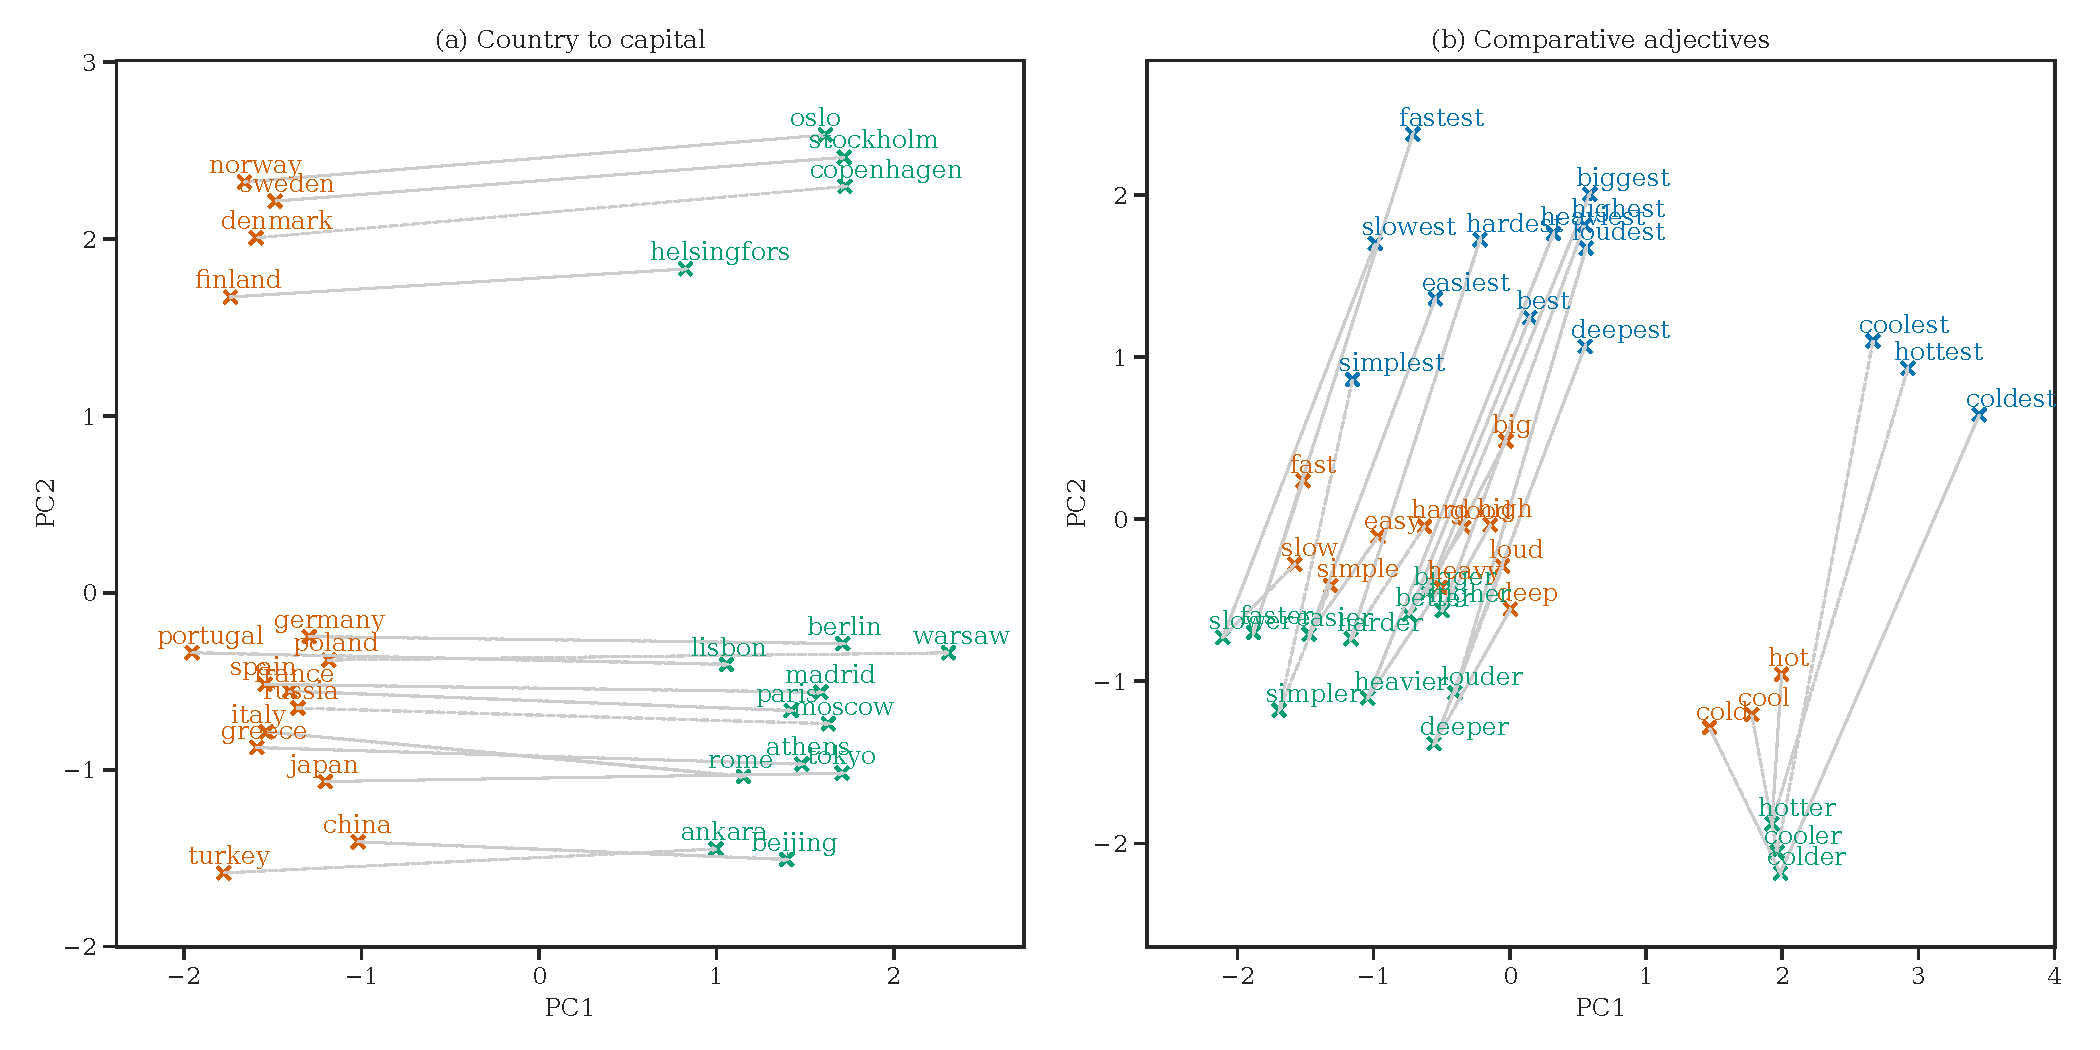
\includegraphics[width=\textwidth]{thesis/figures/word-to-word-relationships-pca-2d.pdf}
 \caption{2-dimensional PCA projection of the word embeddings of SGNS-enwiki of some countries and their capital cities (a) and comparative adjectives (b). This figure is inspired by \cite[Figure 2]{mikolov2013b}.}
 \label{fig:sgns-enwiki-word-to-word-relations-pca-2d}
\end{figure}

Due to the apparent clustering occurring in both plots from \cref{fig:sgns-enwiki-word-to-word-relations-pca-2d}, we investigate the notion of clustering further. In order to understand more about the underlying structure of the SGNS-model, we will in the next section perform cluster analysis of its word embeddings. In particular, we will use multiple clustering algorithms and internal cluster validation methods in order to find the most suitable clustering algorithm and number of clusters.

\section{Word clustering}
In this section, we will apply cluster analysis on the word embeddings of the SGNS-model, in order to search for deeper structures within the data. In the following subsections, we will compare clustering algorithms on the word embeddings of the SGNS-model, and then, look at clustering of distinct groups of words.

\subsection{Comparing clustering algorithms}
\label{sec:comparing-clustering-algorithms}
In this subsection, we compare clustering algorithms on the word embeddings of the SGNS-model. Due to the large number of words in the vocabulary of the SGNS-model (roughly 4.4 million), we restrict the analysis to the 10000 most common (i.e most frequently occurring) words. This way, we speed up the computation by reducing the computational requirement, but should still get a reasonable result, as the most common words yield good quality vector representations (more data $\rightarrow$ better vectors).

To perform the cluster analysis, we use all clustering algorithm from \cref{sec:clustering-algorithms}, except for Spectral clustering (\cref{sec:spectral-clustering}), as it was too computationally expensive for it to run. In particular, we used the following algorithms: k-means clustering (\cref{sec:k-means-clustering}), mini-batch k-means clustering (\cref{sec:mini-batch-k-means-clustering}), k-medoids clustering (\cref{sec:k-medoids-clustering}), GMMs (\cref{sec:gmm-clustering}), hierarchical clustering (agglomerative) (\cref{sec:hierarhical-clustering}), HDBSCAN (\cref{sec:hdbscan-clustering}) and ToMaTo (\cref{sec:tomato-clustering}). We used the \path{scikit-learn} \cite{ScikitLearn2011} and \path{hdbscan} \cite{mcinnes2017hdbscan} pip-packages to perform clustering. Furthermore, we trained each of the clustering algorithms using a grid-search manner, i.e. by trying all combinations of hyperparameters. \cref{table:hyperparameters-clustering-algorithms} shows the hyperparameters used to train each clustering algorithm. By forming a grid of hyperparameters for each clustering algorithm, we get a rough sense for the best set of hyperparameters. For the initial grid-search, we used the same number of clusters for all the algorithms that allows us to specify the number of clusters. Let \path{n_clusters_range}=2, 3, 4, 5, 10, 50, 100, 150, 200, 300, 400, 500, 750, 1000, 1500, 2000, 3000, 4000, 5000, 6000, 7000, 8000 be the range of cluster numbers used for the initial grid-search. We let \path{n_clusters_range} range from 2 to 8000 clusters, using varying step sizes, to investigate the effect of the number of clusters for each algorithm, where it was applicable. To train the clustering algorithm, we use the standard word embeddings if the algorithm supports cosine similarity (or distance) and normalized word embeddings if the algorithm requires Euclidean distances. After training the clustering algorithms, we validated them using the internal cluster validation methods from \cref{sec:cluster-validation}. In particular, we used the mean Silhouette Coefficient (SC)) (\cref{sec:silhouette-coefficient}), the Davies-Bouldin Index (DBI) (\cref{sec:davies-bouldin-index}) and the Caliński-Harabasz Index (CHI) (\cref{sec:calinski-harabasz-index}). We used the \path{scikit-learn} pip-package to perform internal clustering validation.
\begin{table}[H]
    \centering
    \begin{tabular}{@{}ll@{}}
        \toprule
        Clustering algorithm          & Hyperparameters \\
        \midrule
        \trcolor
        K-means clustering            & \makecell[tl]{\path{n_clusters}=\path{n_clusters_range}} \\
        Mini-batch k-means clustering & \makecell[tl]{\path{n_clusters}=\path{n_clusters_range} \\ \path{batch_size}=$100$}\\
        \trcolor
        K-medoids clustering          & \makecell[tl]{\path{n_clusters}=\path{n_clusters_range}}\\
        GMM clustering                & \makecell[tl]{\path{n_components}=\path{n_clusters_range}}\\
        \trcolor
        Agglomerative clustering      & \makecell[tl]{\path{n_clusters}=\path{n_clusters_range} \\ \path{linkage}=[\path{single}, \path{average}, \path{complete}, \path{ward}]}\\
        HDBSCAN                       & \makecell[tl]{\path{min_cluster_size}=$2, 4, 8, 16, 32, 64$ \\ \path{min_samples}=$1, 2, 4, 8, 16, 32, 64$}\\
        \trcolor
        ToMATo                        & \makecell[tl]{\path{density_type}=[\path{DTM}, \path{logDTM}, \path{KDE}, \path{logKDE}] \\ \path{k}=$2, 3, 4, 5, 6, 7, 8, 9, 10, 20, 30, 40, 50, \ldots, 250$}\\ \bottomrule
    \end{tabular}
    \caption{Hyperparameters of clustering algorithms for cluster analysis.}
    \label{table:hyperparameters-clustering-algorithms}
\end{table}

We visualize the result from the initial grid-search in \cref{fig:cluster-analysis-comparison-internal-cluster-validation}. From \cref{fig:cluster-analysis-comparison-internal-cluster-validation}, we see that agglomerative clustering algorithm performs the best (close to k-means clustering) and k-medoids clustering  performs the worst. For this reason, we will now focus on the agglomerative clustering algorithm and search for the best set of hyperparameters, being the linkage criterion and number of clusters.
\begin{figure}[H]
    \centering
    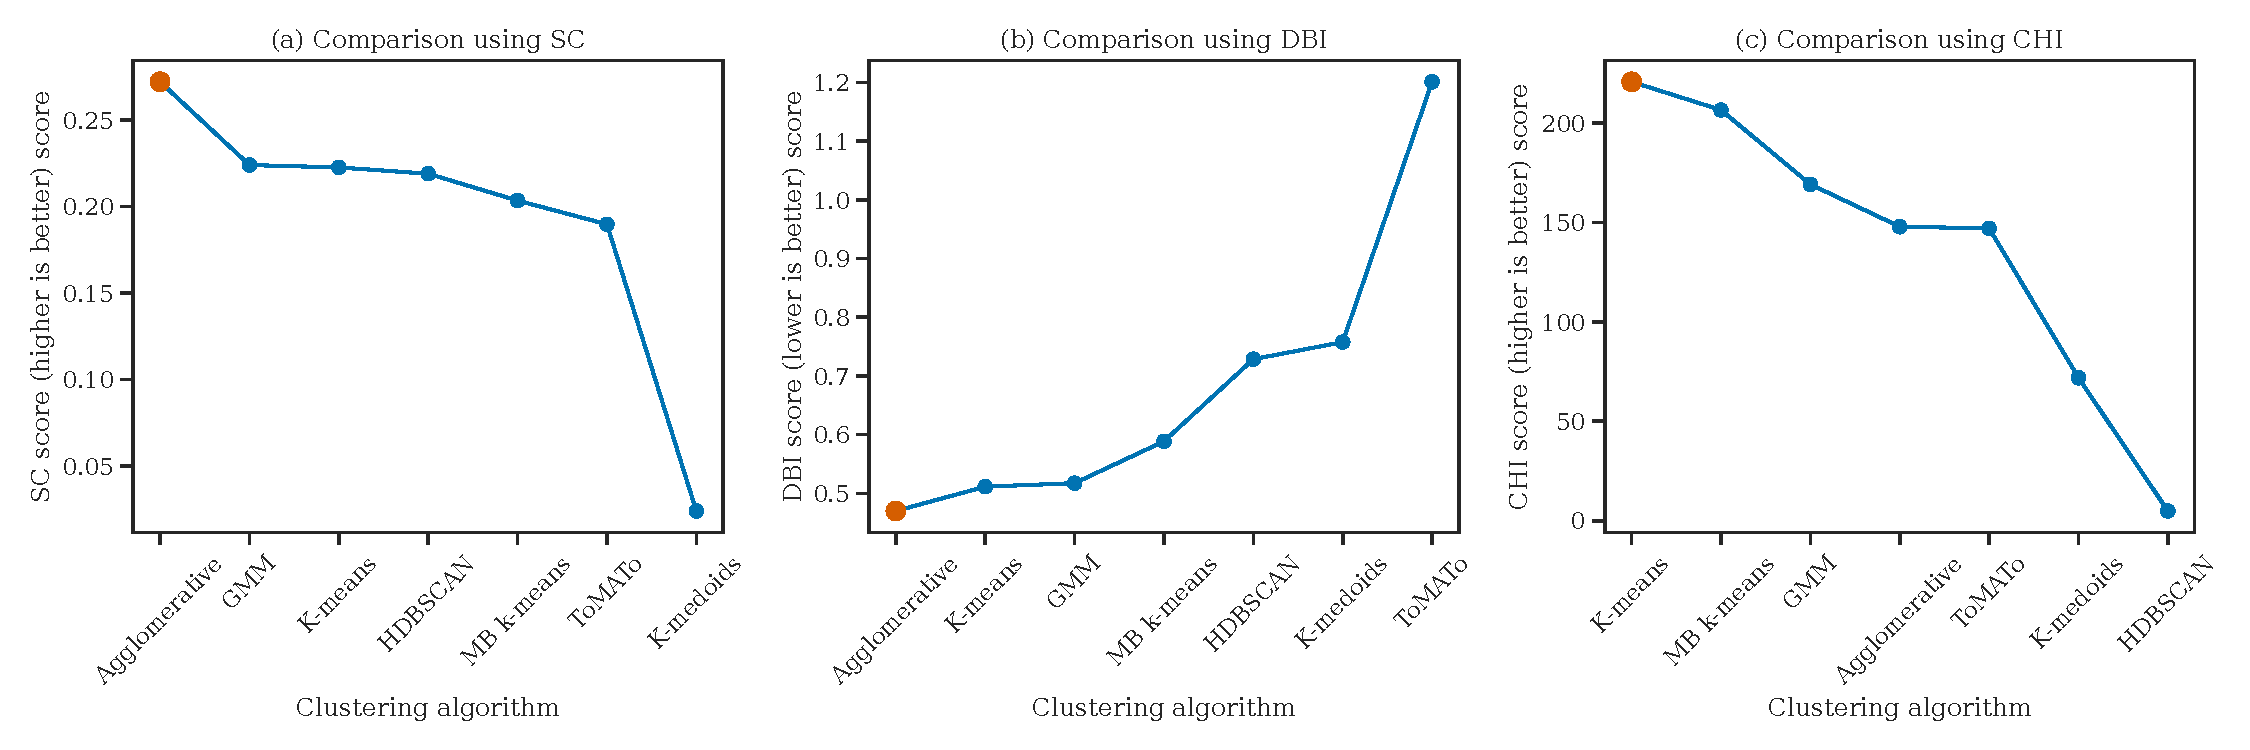
\includegraphics[width=\textwidth]{thesis/figures/cluster-analysis-comparison-internal-cluster-validation.pdf}
    \caption{Comparison of clustering algorithms trained on word embeddings from SGNS-enwiki, ranked by internal cluster validation methods. The red dot in each plot denotes the most optimal value.}
    \label{fig:cluster-analysis-comparison-internal-cluster-validation}
\end{figure}

In order to find the best set of hyperparameters using the agglomerative clustering algorithm, we first visualize its results from the initial grid search in \cref{fig:cluster-analysis-agglomerative-internal-cluster-validation}. From \cref{fig:cluster-analysis-agglomerative-internal-cluster-validation}, first notice that by using the single linkage criterion, we get relatively poor results. The remaining criterions, average, complete and ward, perform more or less the same over all internal clustering validation methods, with the ward criterion being slightly ahead of the rest. By inspecting the best value for the number of clusters for each internal cluster validation method in \cref{fig:cluster-analysis-agglomerative-internal-cluster-validation}, we noticed that the DBI (b) and the CHI (c) gave misleading results, while the SC (a) were more meaningful. In particular, the DBI prefers to have the largest number of clusters, that is, 8000 clusters. We inspected the clusters and observed that 6350 of the words are in its own cluster of size 1. This means that the DBI is not particularly well suited for choosing the number of clusters, as it prefers to have the most clusters. This is also illustrated by looking at the plot in the middle (b) of \cref{fig:cluster-analysis-agglomerative-internal-cluster-validation}. Using the CHI, we observe that it prefers to have the least number of clusters, namely 2. We inspected this result, and noticed that in the first clusters, there were only a single word, while the second cluster had the remaining 9999 words. In other words, this means that the CHI is also not particularly well suited for choosing the number of clusters. Finally, using the SC (a), we observe that the preferred number of clusters lie around 3000 to 6000. We inspected the number of clusters as preferred by average, complete and ward linkage clustering and concluded that they made sense, as there were more variety in the cluster sizes and the number of clusters having the specific each cluster sizes. This indicates that the most preferable number of clusters (using SC) should lie in this range (3000 to 6000), and following, we will narrow down the search for the best number of clusters. For the next experiment, we will not include the single linkage clustering criterion, as it performed poorly.
\begin{figure}[H]
    \centering
    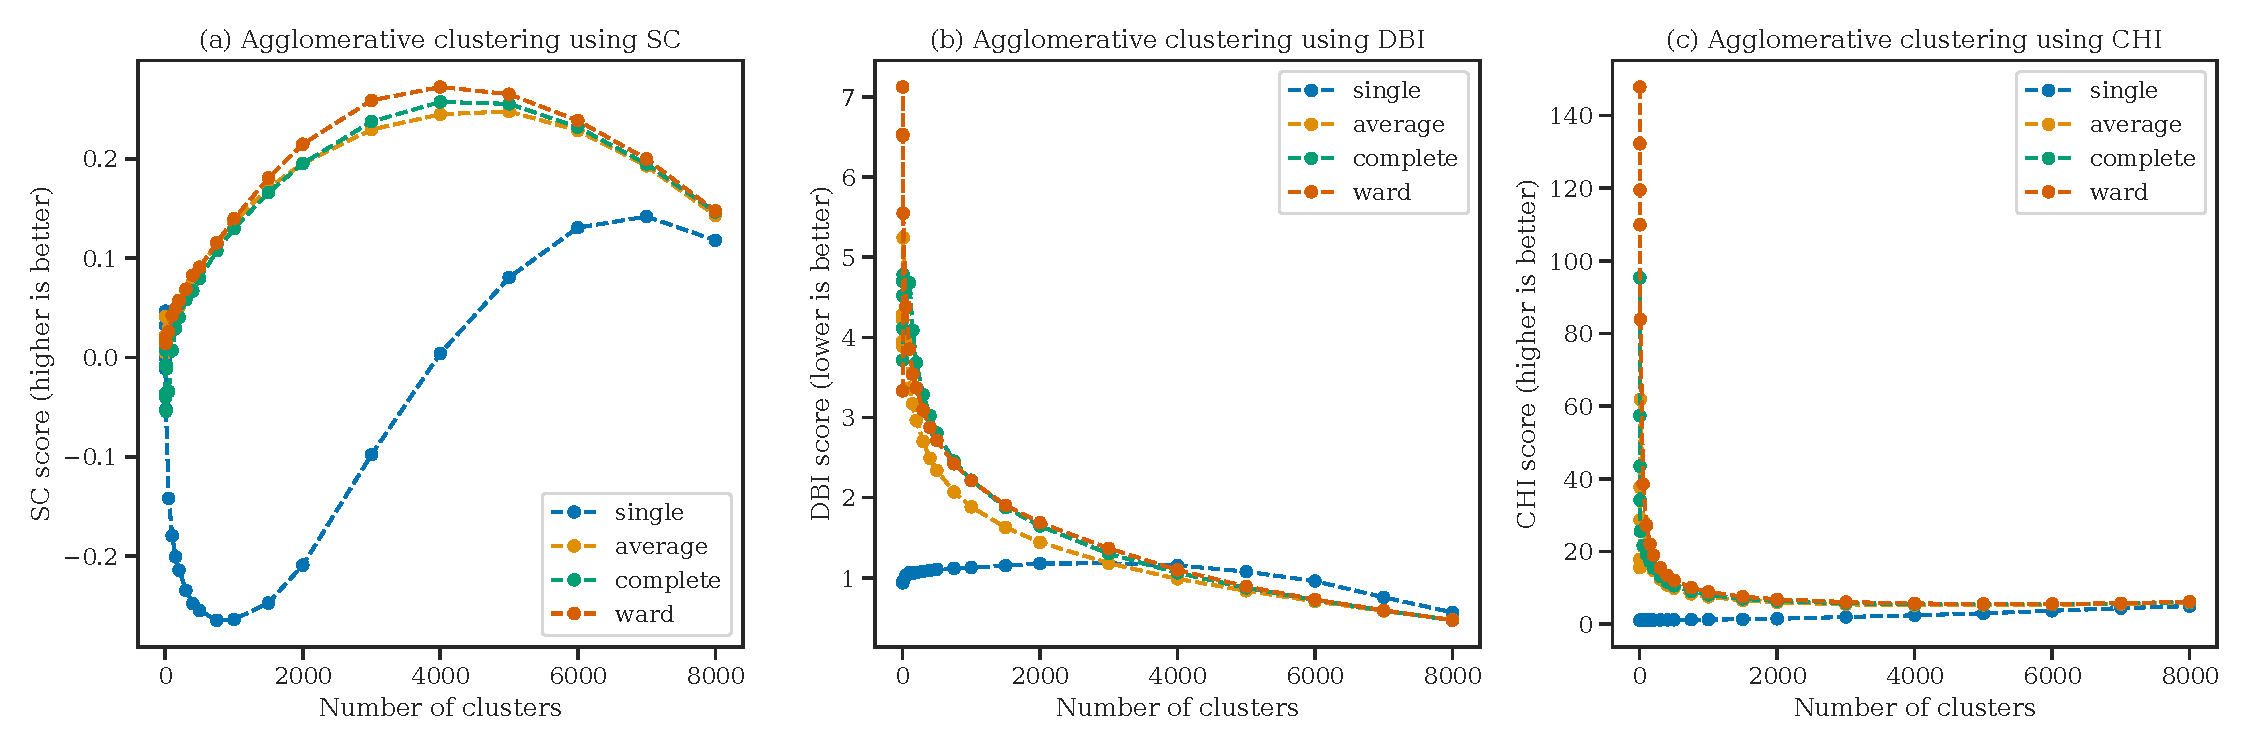
\includegraphics[width=\textwidth]{thesis/figures/cluster-analysis-agglomerative-internal-cluster-validation.pdf}
    \caption{Internal cluster validation results using agglomerative clustering on word embeddings from SGNS-enwiki.}
    \label{fig:cluster-analysis-agglomerative-internal-cluster-validation}
\end{figure}

By narrowing the search to the range 3000 to 6000 clusters, we find the best number of clusters for each criterion, using agglomerative clustering. The narrowed search for number of clusters is shown in \cref{fig:cluster-analysis-agglomerative-internal-cluster-validation-narrow}, and we observe that ward linkage clustering with 4104 clusters result in the best clustering of the 10000 most common words from the SGNS-enwiki model.
\begin{figure}[H]
    \centering
    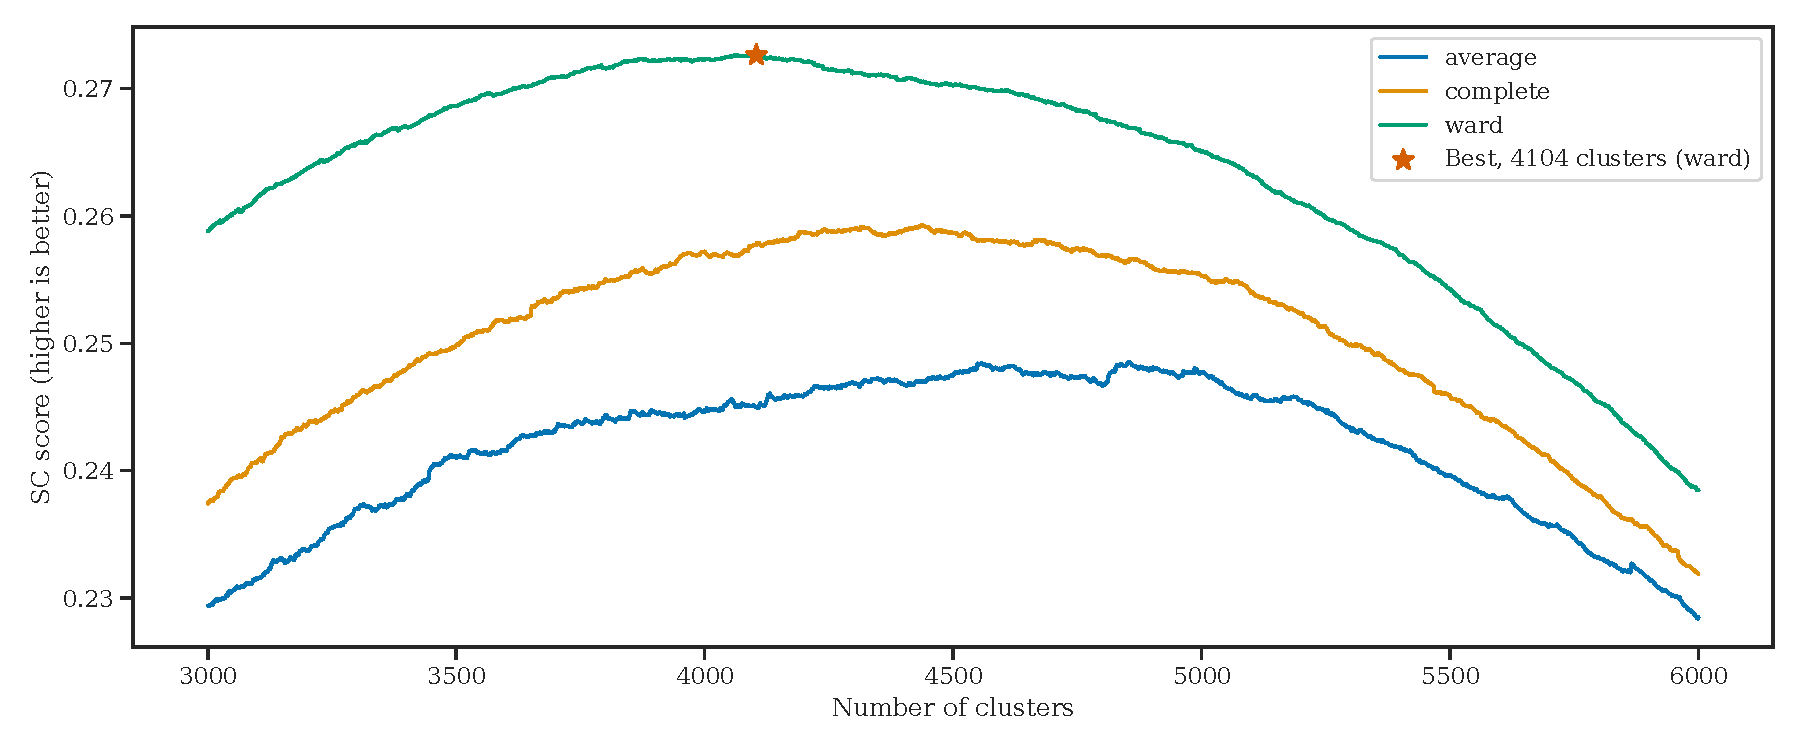
\includegraphics[width=\textwidth]{thesis/figures/cluster-analysis-agglomerative-internal-cluster-validation-narrow.pdf}
    \caption{Number of clusters search using agglomerative clustering and SC, on the range of 3000 to 6000 clusters. Here we see that ward linkage criterion results in the highest SC score.}
    \label{fig:cluster-analysis-agglomerative-internal-cluster-validation-narrow}
\end{figure}

To further gain knowledge of what the best clustering using agglomerative clustering on the word embeddings from SGNS-enwiki, we investigate the words falling into the 4104 clusters, with agglomerative clustering and ward criterion. In particular, we look at the 10 largest and smallest clusters. For the smallest clusters, we look at clusters of size 2 or more, to ensure we do not have clusters consisting of single words. In the top 10 largest clusters, we mostly see names such as "Smith", "Wilson" or "Taylor" being clustered into the same cluster. We also see words representing numbers being clustered together, e.g. "forty-five", "thirty-two" or "fifty-one", and family related words being clustered together, e.g. "father", "son" and "brother". The top 10 smallest clusters mostly consist of words that are strongly related to one another, such as "Adam" and "Noah", "card" and "cards", or "interior" and "exterior". We visualize some of the largest and smallest clusters in \cref{fig:cluster-analysis-agglomerative-2d-umap-top-clusters}, using a 2-dimensional UMAP (\cref{sec:umap}) embedding. To create the UMAP embedding, we used the \path{umap-learn} pip-package \cite{mcinnes2018umap-software}, and let \path{n_neighbors=15} and \path{min_dist=0.1}. From \cref{fig:cluster-analysis-agglomerative-2d-umap-top-clusters}, we see that the clusters are widely spread all over the UMAP embedding. In addition to this, the UMAP embedding suggests that there are more clusters throughout the word embeddings, which the clustering algorithms simply were unable to pick up (when evaluated using internal cluster validation methods). We will investigate this further, and in the next subsection, we will look at clustering of distinct word groups. In particular, we will see if bigger sets of words cluster together in the UMAP embedding, suggesting that the word embeddings contains deeper structure.
\begin{figure}
    \centering
    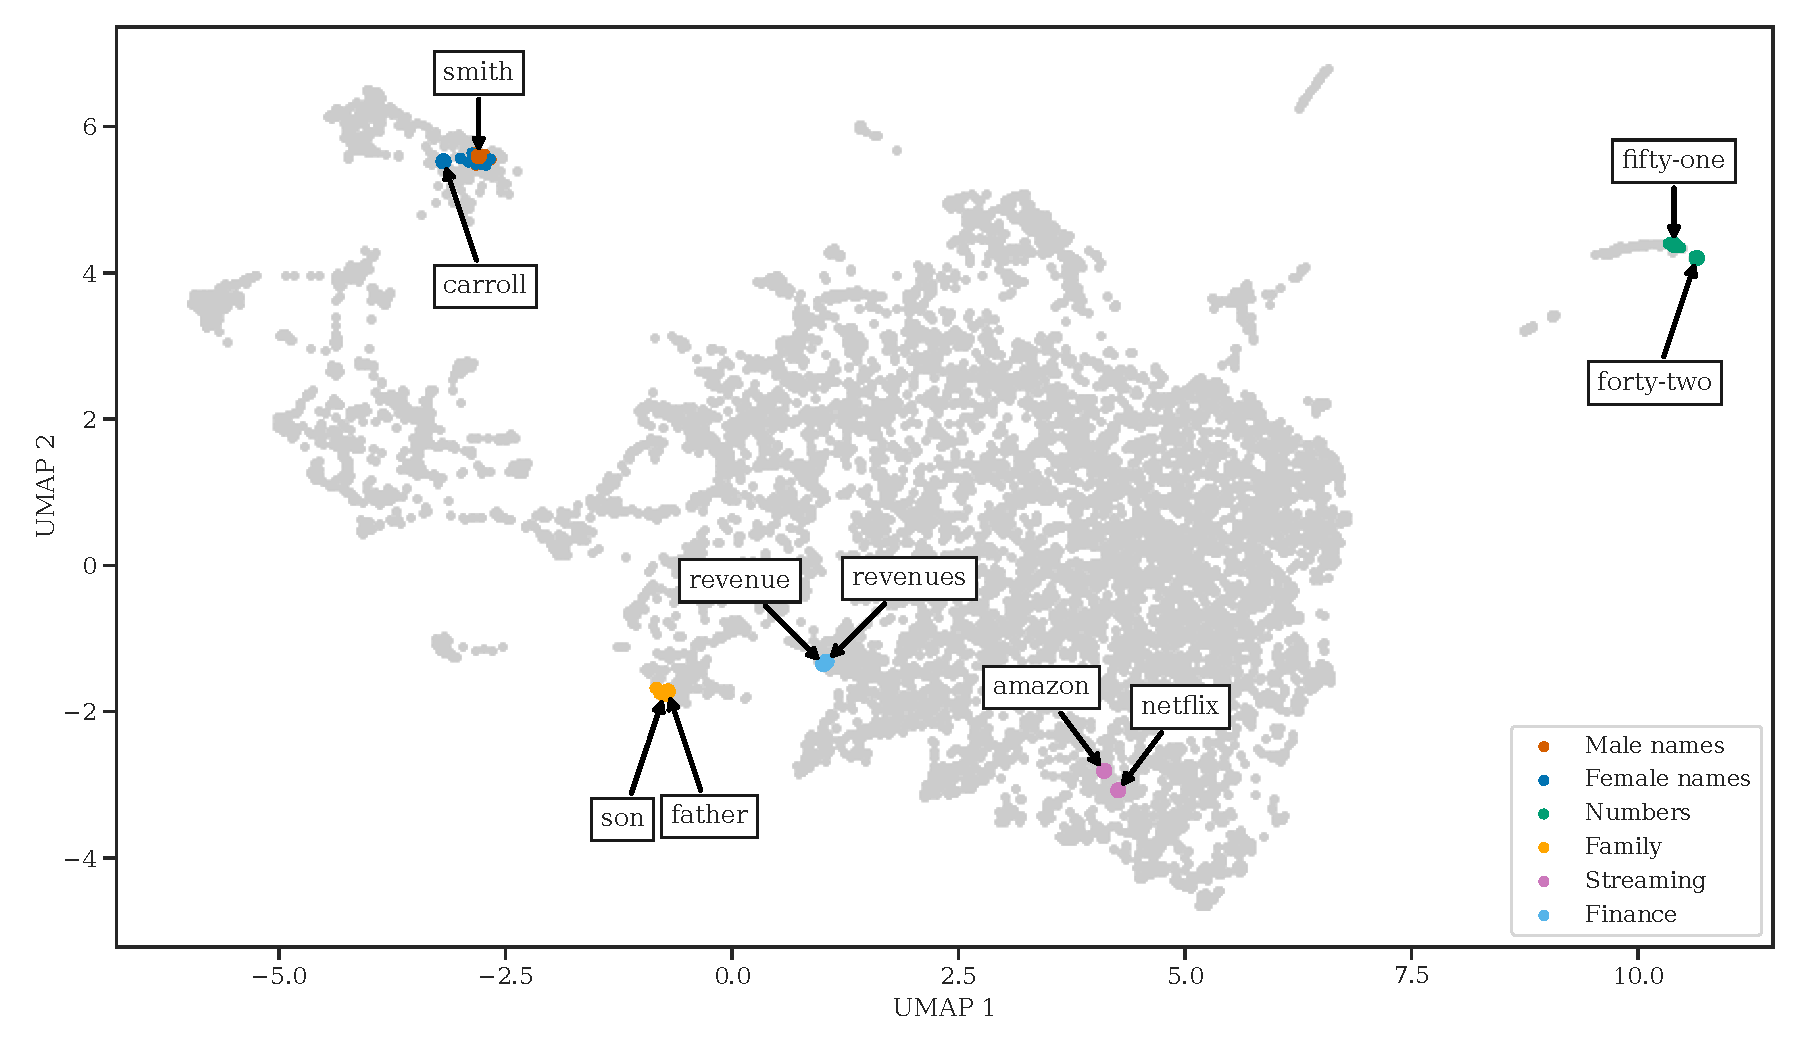
\includegraphics[width=\textwidth]{thesis/figures/cluster-analysis-agglomerative-2d-umap-top-clusters.pdf}
    \caption{2-dimensional UMAP embedding of the 10000 most common words from the SGNS-enwiki model, with some of the largest/smallest clusters outlined.}
    \label{fig:cluster-analysis-agglomerative-2d-umap-top-clusters}
\end{figure}

\subsection{Clustering word groups}
In this subsection, we will investigate the effect of clustering in the 2-dimensional UMAP embedding of the 10000 most common words of the SGNS-enwiki model, using distinct groups of words. In particular, we will cluster words related to countries/capitals, numbers, names (fore- and surnames) and food. Prior to performing the clustering, we first prepare the data to be used for the analysis. The countries/capitals data was retrieved from \cite{GeoNames}, where we used their API in order to fetch countries and its capital, resulting in 217 pairs of countries and capitals that were in the SGNS-enwiki vocabulary. The number data was generated by converting numbers to its string representation. We converted the numbers from zero to one trillion, resulting in 105 number related words. The forenames data was retrieved from \cite{SSABabyNames}, where we used the top 1000 baby names from 2019. The surnames data was retrieved from \cite{CensusSurnames}, and we used the top 1000 surnames from 2010. Finally, the food data was retrieved from \cite{FoodIngredientList}, where we used the 250 most common ingredient words. We visualize the largest clusters of word groups falling into the 10000 most common words from the SGNS-enwiki word embeddings, embedded into a 2-dimensional UMAP embeddings in \cref{fig:word-cluster-all-groups}. From \cref{fig:word-cluster-all-groups}, we observe that there are two well separated clusters forming in the UMAP embedding, namely the names and numbers word groups. The countries and food groups are more spread out in the embedding.
\begin{figure}[H]
    \centering
    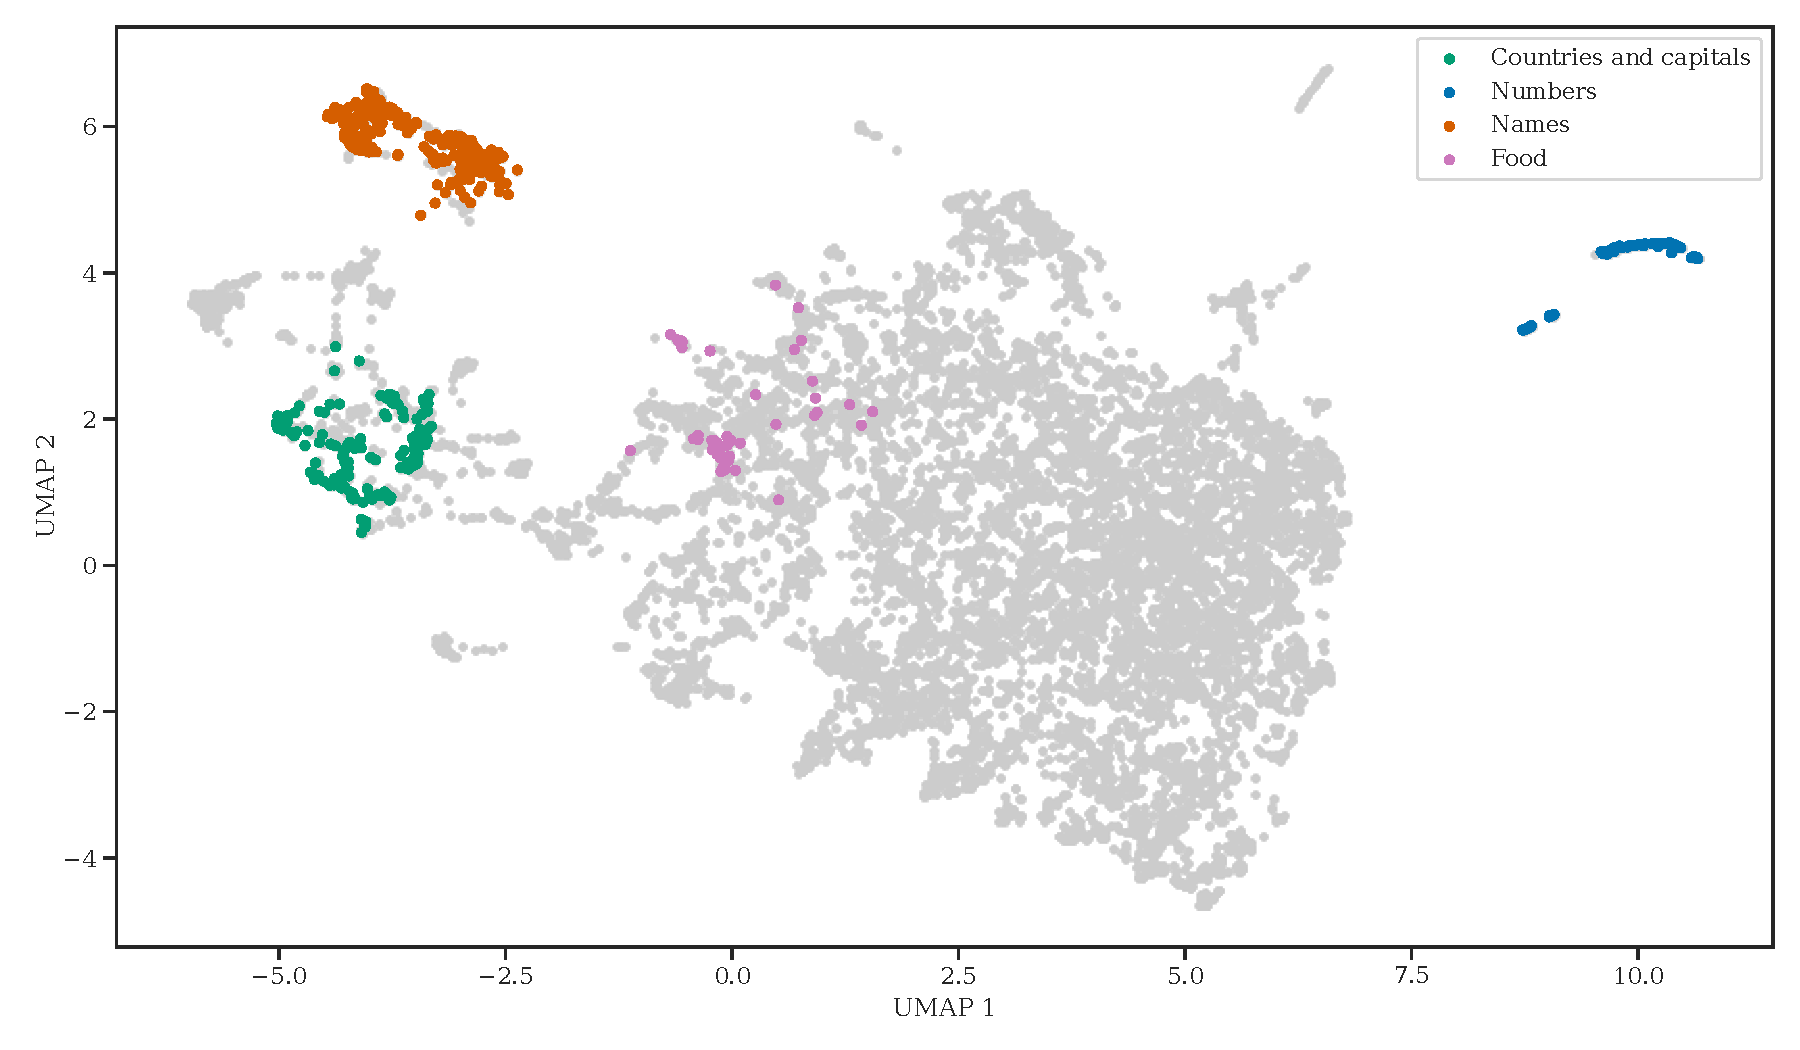
\includegraphics[width=\textwidth]{thesis/figures/word-cluster-all-groups.pdf}
    \caption{2-dimensional UMAP embedding of the 10000 most common words from the SGNS-enwiki model, with word groups outlined.}
    \label{fig:word-cluster-all-groups}
\end{figure}

Note that, in \cref{fig:word-cluster-all-groups}, we have outlined the largest clusters of the word groups, and discarded words falling out of the largest clusters. By including words that are outside the largest clusters, we saw that, in particular, the names word group is spread throughout the word embedding, as the data we used contained fore- and surnames of common words, such as "joy", "page" or "good". We illustrate this behaviour in \cref{fig:word-cluster-all-groups-emphasis-plots}, where we outline the four different word groups. From \cref{fig:word-cluster-all-groups-emphasis-plots}, we see that the country and capital words (a) are mostly clustered to the middle left, with some capitals falling out of the bigger cluster. The "Stanley" and "Hamilton" capital cities are also used as names, indicated by the names (c) plot. For the numbers, we observe that most number related words are clustered to the right, clearly separated from the rest of the words. However, we also observe that words such as "million", "billion" and "trillion" are clustered together outside the numbers cluster to the right. By inspection, we observed that the "million", "billion" and "trillion" words were in fact close to other financial words, such as "banks", "wealth" or "economics". For the names (c), we see that the fore- and surnames are clustered to the top right, but also spread throughout the UMAP embedding. We also observe a small cluster of woman names forming, containing the names "Diana" and "Isabella". Lastly, we see that food related words (d) are slightly clustered around the words "egg" and "cheese", but also slightly spread around the UMAP embedding. An interesting observation is the word "apple", which is both a fruit and a technology company. In this case, the word apple refers to the company Apple Inc., as we also saw earlier in \cref{table:word2vec-nearest-neighbours-words}.
\begin{figure}[H]
    \centering
    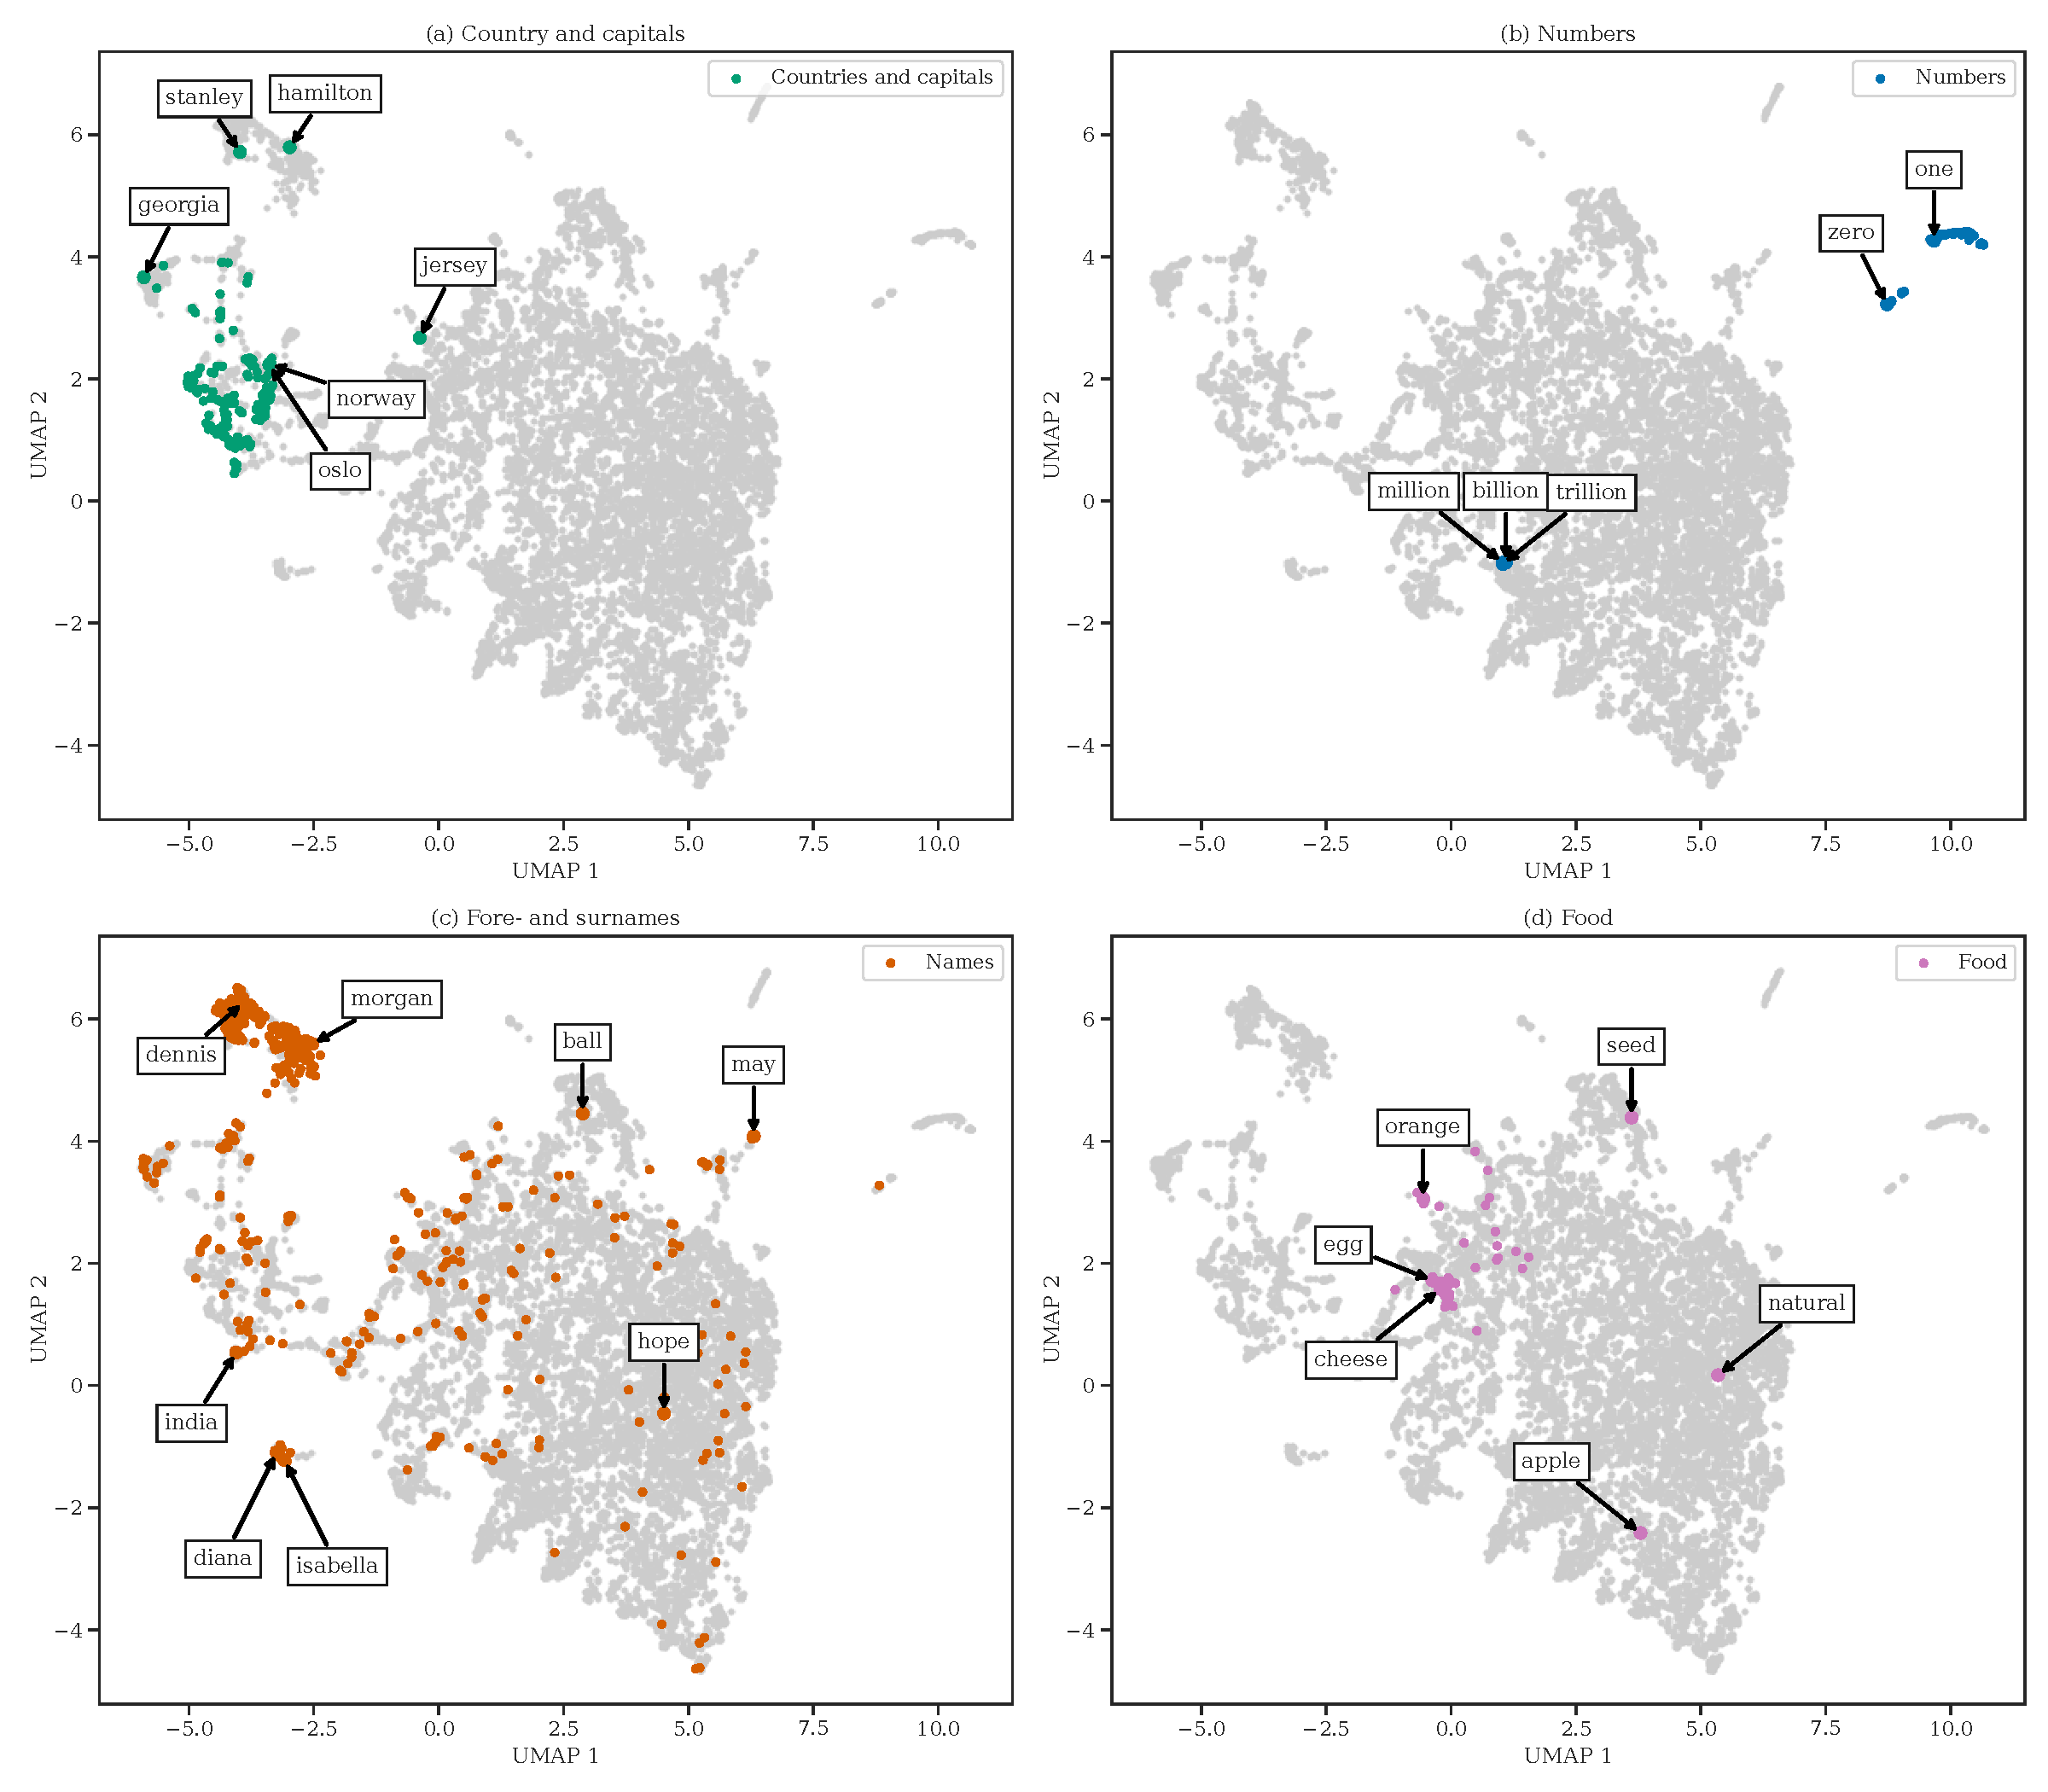
\includegraphics[width=\textwidth]{thesis/figures/word-cluster-all-groups-emphasis-plots.pdf}
    \caption{2-dimensional UMAP embeddings of the 10000 most common words from the SGNS-enwiki model. Here we see four plots, where in each plot we have outlined the four different word groups.}
    \label{fig:word-cluster-all-groups-emphasis-plots}
\end{figure}

We will now further analyze two of the word groups to further develop our understanding of the word embeddings. In particular, we will perform cluster analysis of the word embeddings of countries/capitals and numbers, where we will use clustering algorithms to cluster the words. We will use the same clustering algorithms specified in \cref{sec:comparing-clustering-algorithms}, in addition to Spectral clustering. In order to visualize the results, we will use dimensionality reduction algorithms to create 2-dimensional embeddings. We will also use latitude/longitude coordinates of countries in order to visualize the clustering results using countries/capitals word embeddings.

We analyze the countries and capital word groups separately, as we choose to either identify a country by its name or its capital. Starting with the country word group, we perform cluster analysis. The result of the cluster analysis is summarized in \cref{fig:cluster-analysis-country-word-group-internal-cluster-validation}. There we see a similar result to the result shown in \cref{fig:cluster-analysis-comparison-internal-cluster-validation}, namely that agglomerative clustering is the preferred choice of clustering algorithm.
\begin{figure}[H]
    \centering
    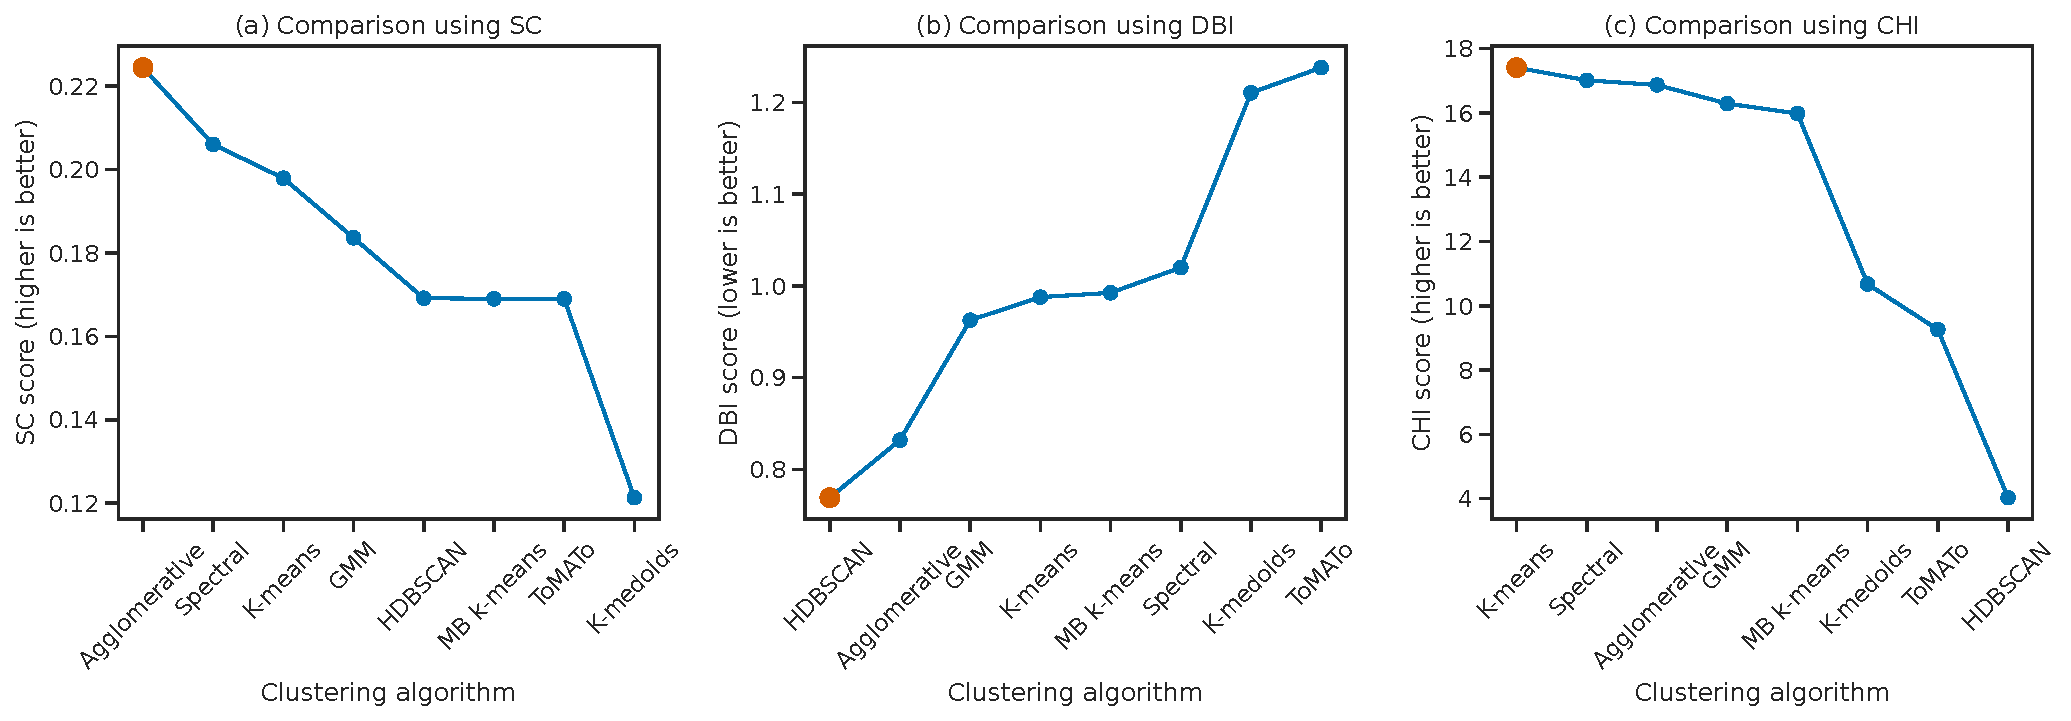
\includegraphics[width=\textwidth]{thesis/figures/cluster-analysis-country-word-group-internal-cluster-validation.pdf}
    \caption{Comparison of clustering algorithms trained on country word embeddings from SGNS-enwiki, ranked by internal cluster validation methods. The red dot in each plot denotes the most optimal value.}
    \label{fig:cluster-analysis-country-word-group-internal-cluster-validation}
\end{figure}

Following, we inspected the scores from the DBI and CHI methods and observed a similar pattern to the analysis from \cref{sec:comparing-clustering-algorithms}, namely that DBI prefers every word to be in its own cluster and CHI prefers to have the smallest number of clusters (i.e. 2). For this reason, we mainly focus on the results using SC. Using agglomerative clustering, we visualize its result in \cref{fig:cluster-analysis-agglomerative-country-word-group-internal-cluster-validation}. From \cref{fig:cluster-analysis-agglomerative-country-word-group-internal-cluster-validation}, we see similar results to \cref{fig:cluster-analysis-agglomerative-internal-cluster-validation}, namely that ward criterion gives the best clustering when using agglomerative clustering.
\begin{figure}[H]
    \centering
    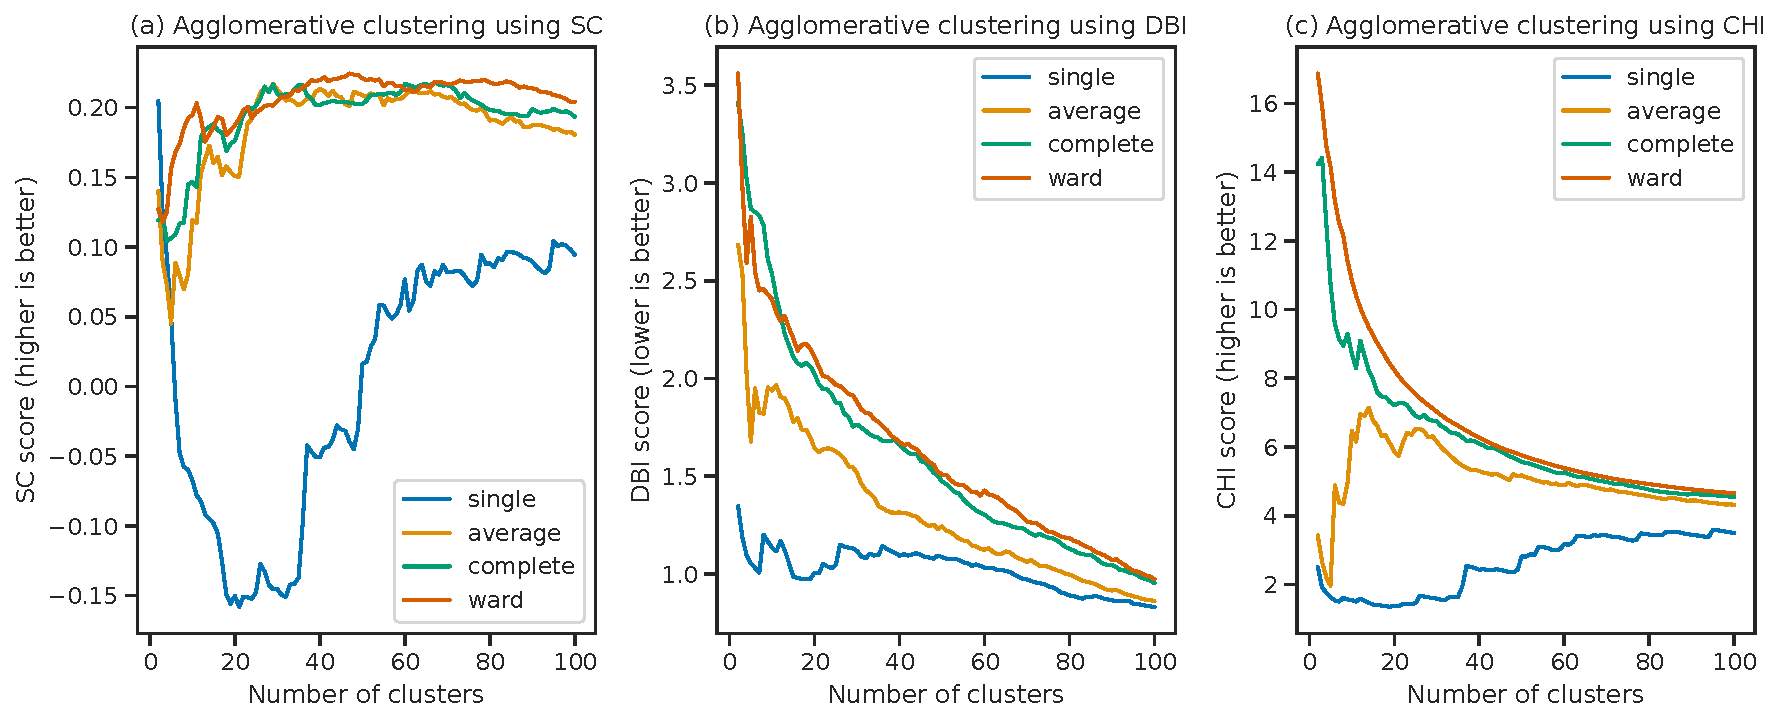
\includegraphics[width=\textwidth]{thesis/figures/cluster-analysis-agglomerative-country-word-group-internal-cluster-validation.pdf}
    \caption{Internal cluster validation results using agglomerative clustering on country word embeddings from SGNS-enwiki.}
    \label{fig:cluster-analysis-agglomerative-country-word-group-internal-cluster-validation}
\end{figure}

The best clustering using SC with agglomerative clustering and ward criterion resulted in 47 clusters. We visualize this result using latitude/longitude coordinates of each country by emphasizing the five largest clusters in \cref{fig:cluster-analysis-agglomerative-country-word-group-top-clusters}. From \cref{fig:cluster-analysis-agglomerative-country-word-group-top-clusters}, we see that the top 5 largest clusters are clustered together in the same continent.
\begin{figure}[H]
    \centering
    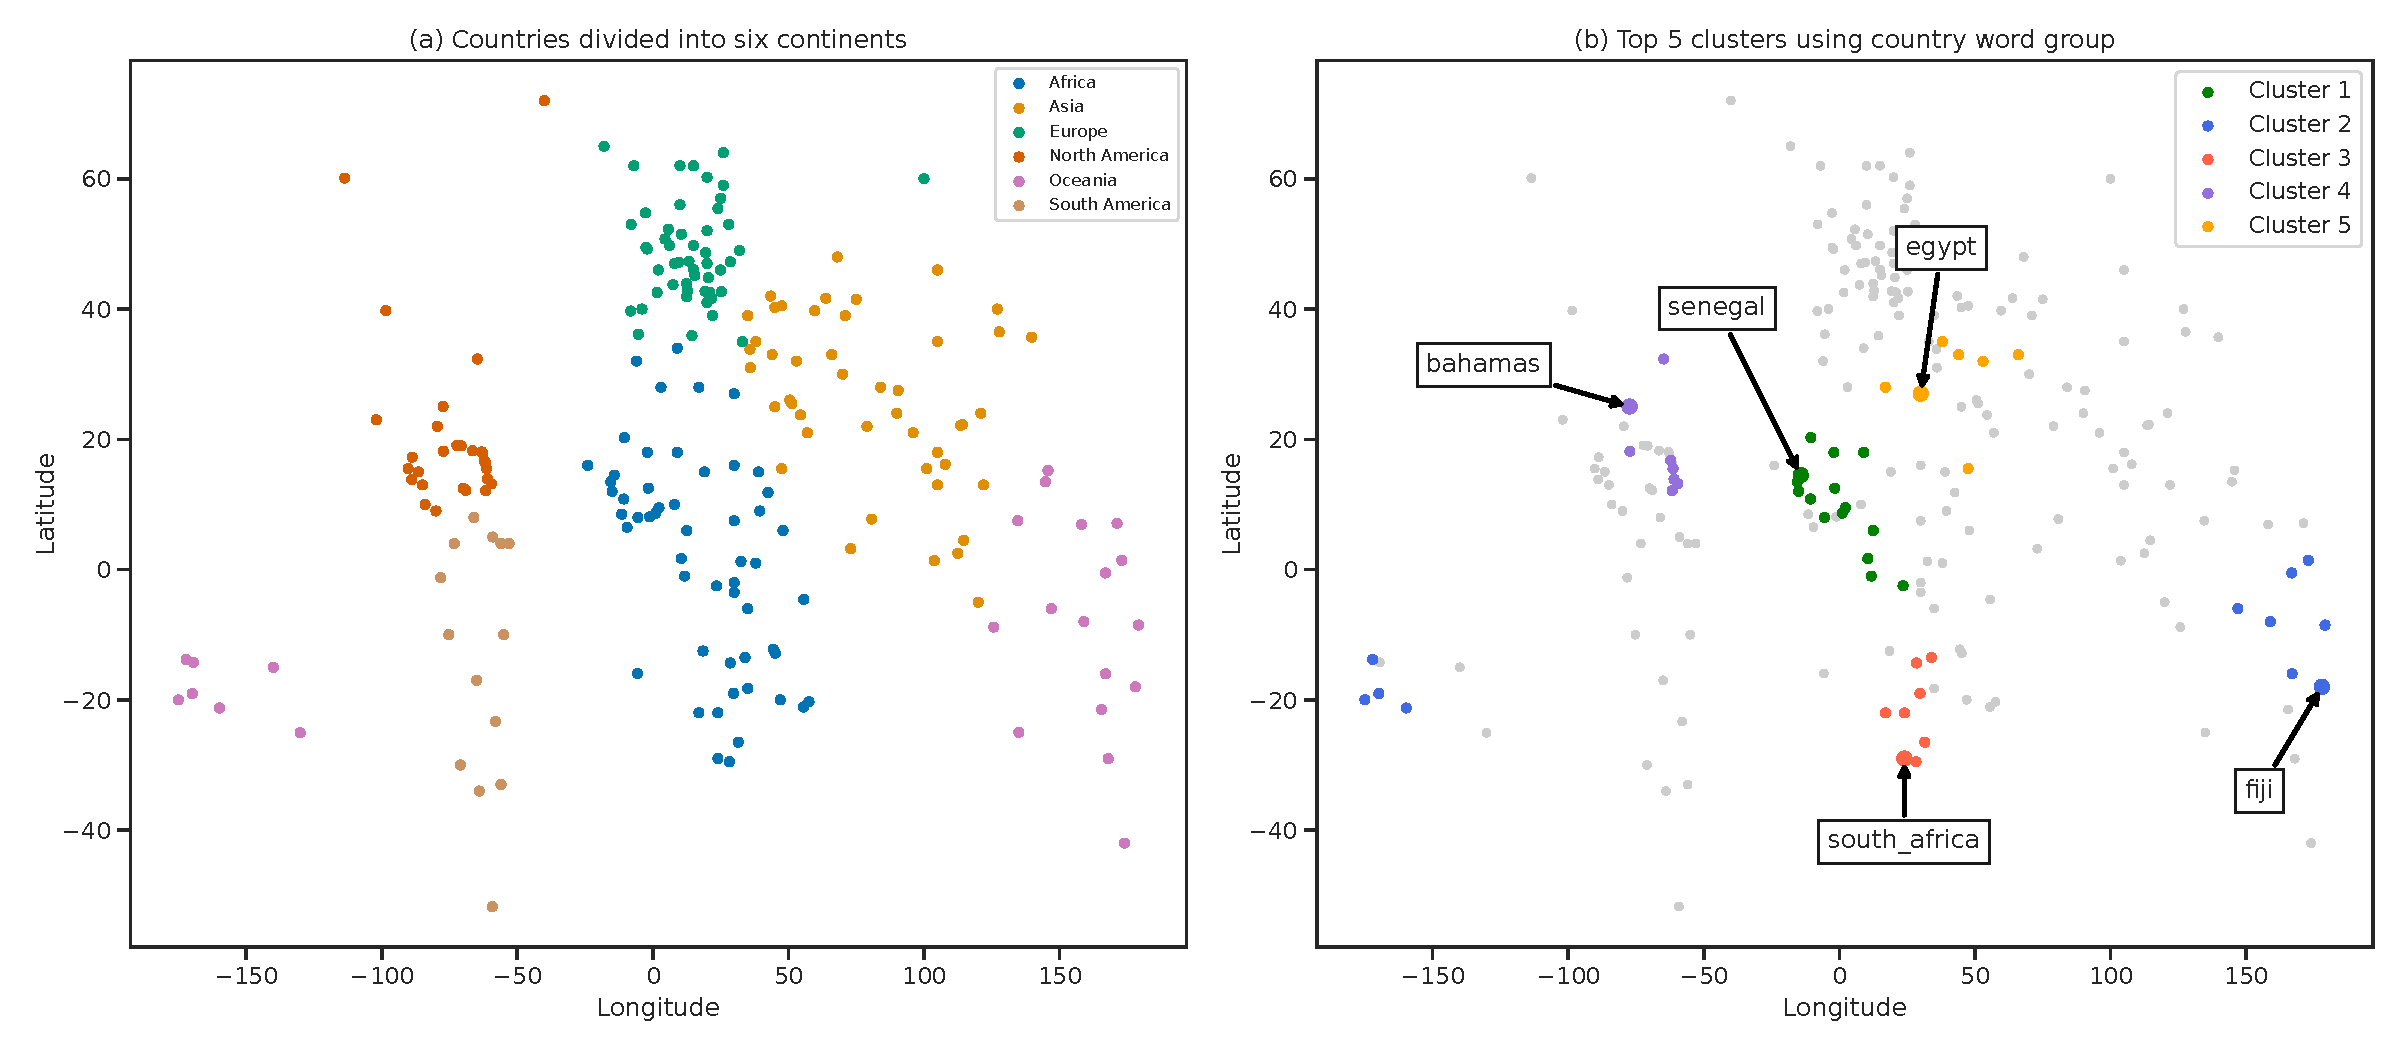
\includegraphics[width=\textwidth]{thesis/figures/cluster-analysis-agglomerative-country-word-group-top-clusters.pdf}
    \caption{Comparison of countries clustered into their respective continents (a) versus top 5 largest clusters from clustering of country word embeddings from SGNS-enwiki using agglomerative clustering and ward criterion. Here we can see that the top 5 largest clusters using agglomerative clustering correlate well with the continent of the respective countries.}
    \label{fig:cluster-analysis-agglomerative-country-word-group-top-clusters}
\end{figure}

Furthermore, we repeat the cluster analysis using capital to identify each country. That is, we use the word embeddings of the capital words instead of the previously used country word embeddings. The result of the cluster analysis is summarized in \cref{fig:cluster-analysis-country-capitals-word-group-internal-cluster-validation}. There we see a similar result to the result shown in both \cref{fig:cluster-analysis-comparison-internal-cluster-validation} and \cref{fig:cluster-analysis-country-word-group-internal-cluster-validation}, namely that agglomerative clustering is the preferred choice of clustering algorithm.
\begin{figure}[H]
    \centering
    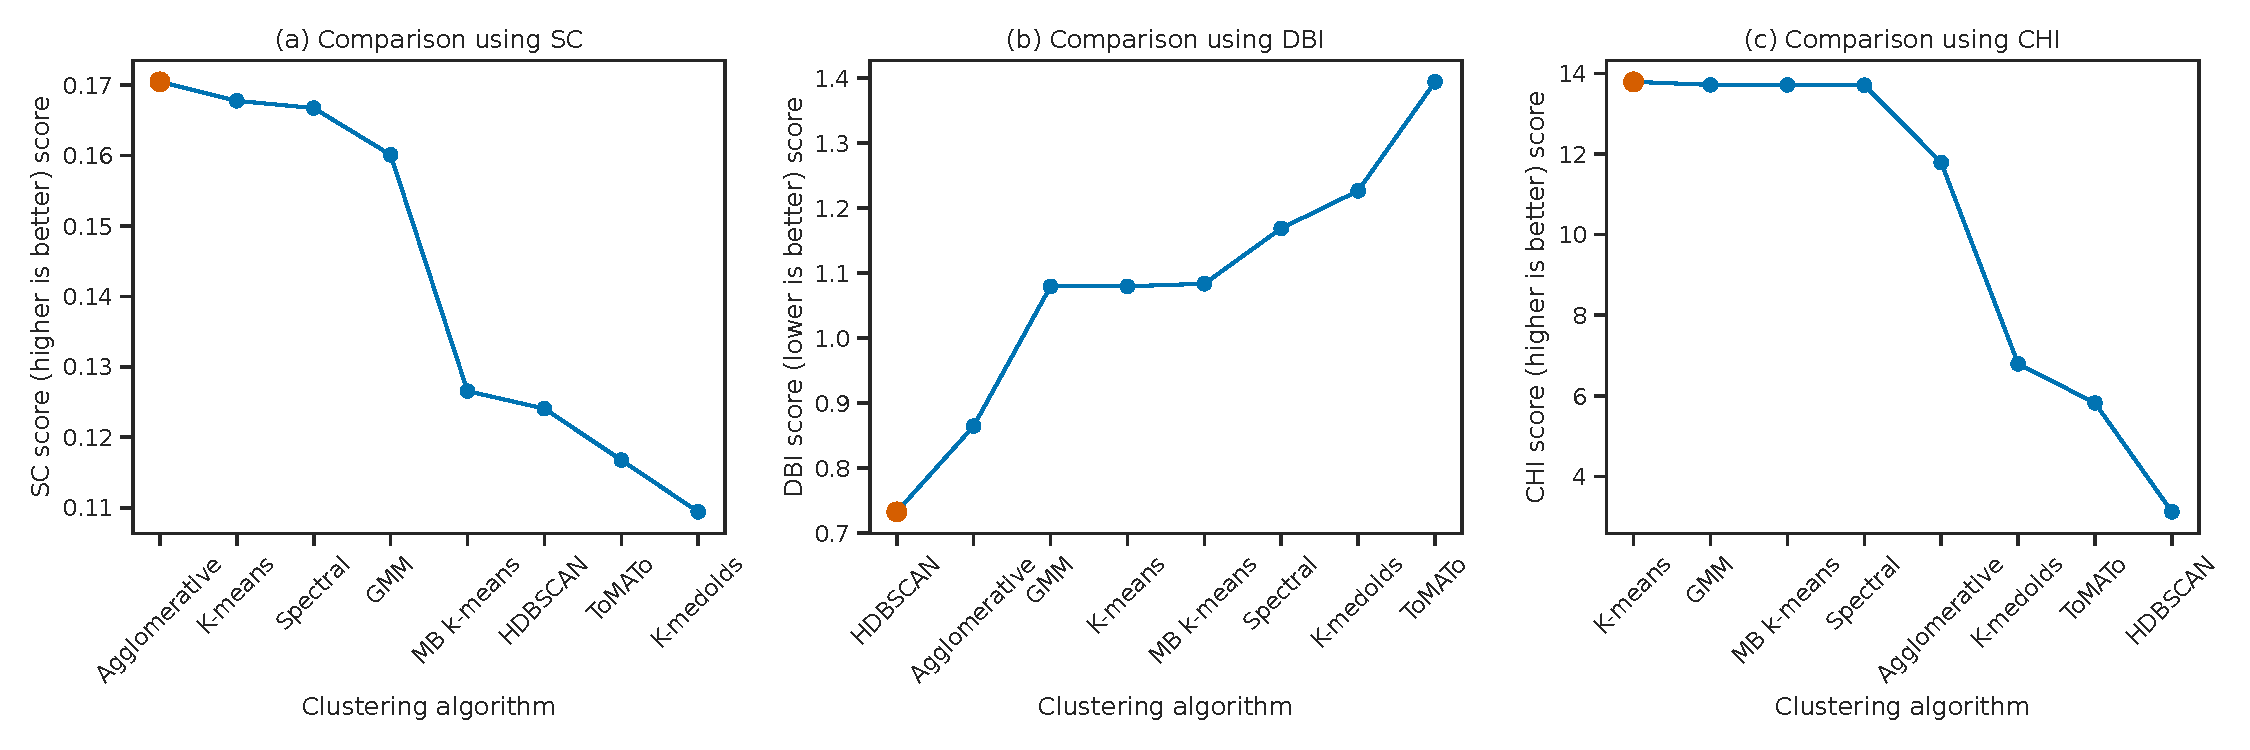
\includegraphics[width=\textwidth]{thesis/figures/cluster-analysis-country-capitals-word-group-internal-cluster-validation.pdf}
    \caption{Comparison of clustering algorithms trained on capital word embeddings from SGNS-enwiki, ranked by internal cluster validation methods. The red dot in each plot denotes the most optimal value.}
    \label{fig:cluster-analysis-country-capitals-word-group-internal-cluster-validation}
\end{figure}

We inspected the scores from the DBI and CHI methods, and similar to the results from \cref{sec:comparing-clustering-algorithms} and the cluster analysis using country word embeddings, we saw that DBI prefers every word to be in its own cluster and CHI prefers to have the smallest number of clusters (i.e. 2). This further strengthens the motivation to use SC over the other methods, and we mainly focus on the results using SC. Using agglomerative clustering, we visualize the results using capital word embeddings in \cref{fig:cluster-analysis-agglomerative-country-capitals-word-group-internal-cluster-validation}. From \cref{fig:cluster-analysis-agglomerative-country-capitals-word-group-internal-cluster-validation}, we see similar results to \cref{fig:cluster-analysis-agglomerative-internal-cluster-validation} and \cref{fig:cluster-analysis-agglomerative-country-word-group-internal-cluster-validation}, namely that ward criterion gives the best clustering when using agglomerative clustering.
\begin{figure}[H]
    \centering
    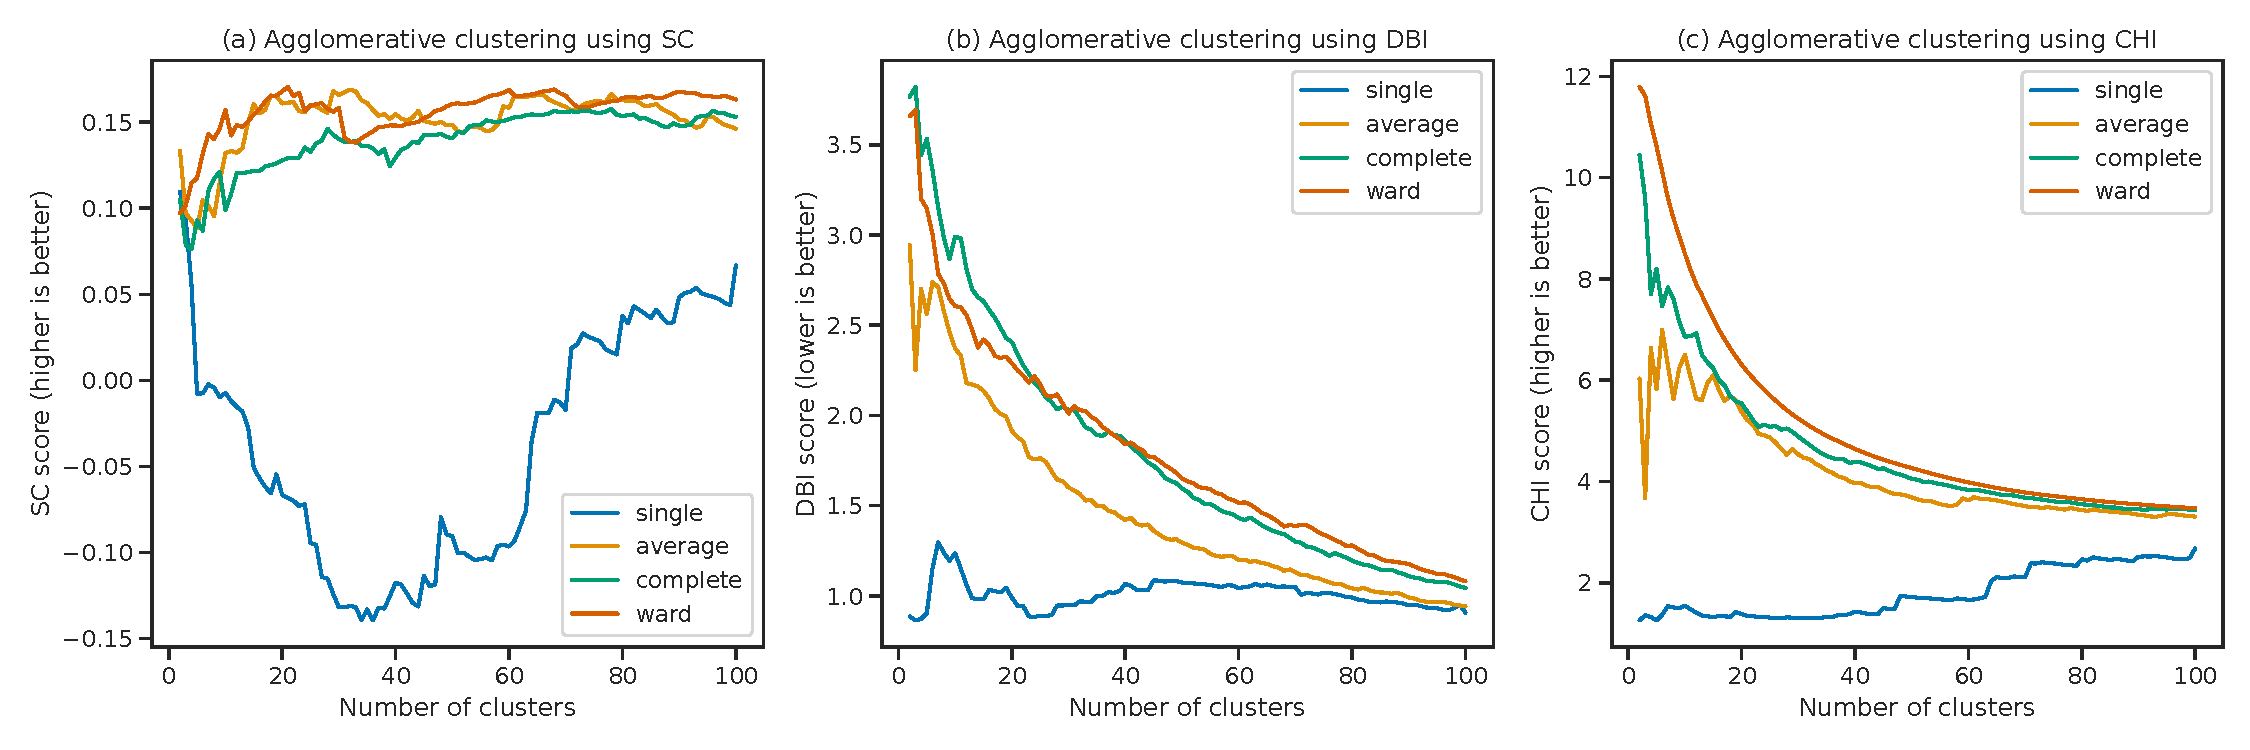
\includegraphics[width=\textwidth]{thesis/figures/cluster-analysis-agglomerative-country-capitals-word-group-internal-cluster-validation.pdf}
    \caption{Internal cluster validation results using agglomerative clustering on capital word embeddings from SGNS-enwiki.}
    \label{fig:cluster-analysis-agglomerative-country-capitals-word-group-internal-cluster-validation}
\end{figure}

The best clustering using SC with agglomerative clustering and ward criterion resulted in 21 clusters. We visualize this result using latitude/longitude coordinates of each country by emphasizing the five largest clusters in \cref{fig:cluster-analysis-agglomerative-country-capitals-word-group-top-clusters}. From \cref{fig:cluster-analysis-agglomerative-country-capitals-word-group-top-clusters}, we see that we get larger clusters than by using country word embeddings in \cref{fig:cluster-analysis-agglomerative-country-word-group-top-clusters}. Furthermore, we observe that in plot (b) the first cluster (green) consists of capitals where the countries are Spanish talking, as outlined by the "Madrid" (Spain), "Mexico City" (Mexico) and "Santiago" (Chile) boxes. The second cluster (blue) in plot (b) also correlates well with the Oceanic continent of plot (a), while the third (red) and forth (purple) clusters of plot (b) seem to capture the African continent very well (Dakar is the capital of Senegal and Pretoria is one of the capitals of South Africa). The last cluster (yellow) consists of capitals from Eastern Europe, as well as some Asian capitals. This concludes the cluster analysis of country and capital word embeddings, and furthermore, we will perform cluster analysis of words related to numbers.
\begin{figure}[H]
    \centering
    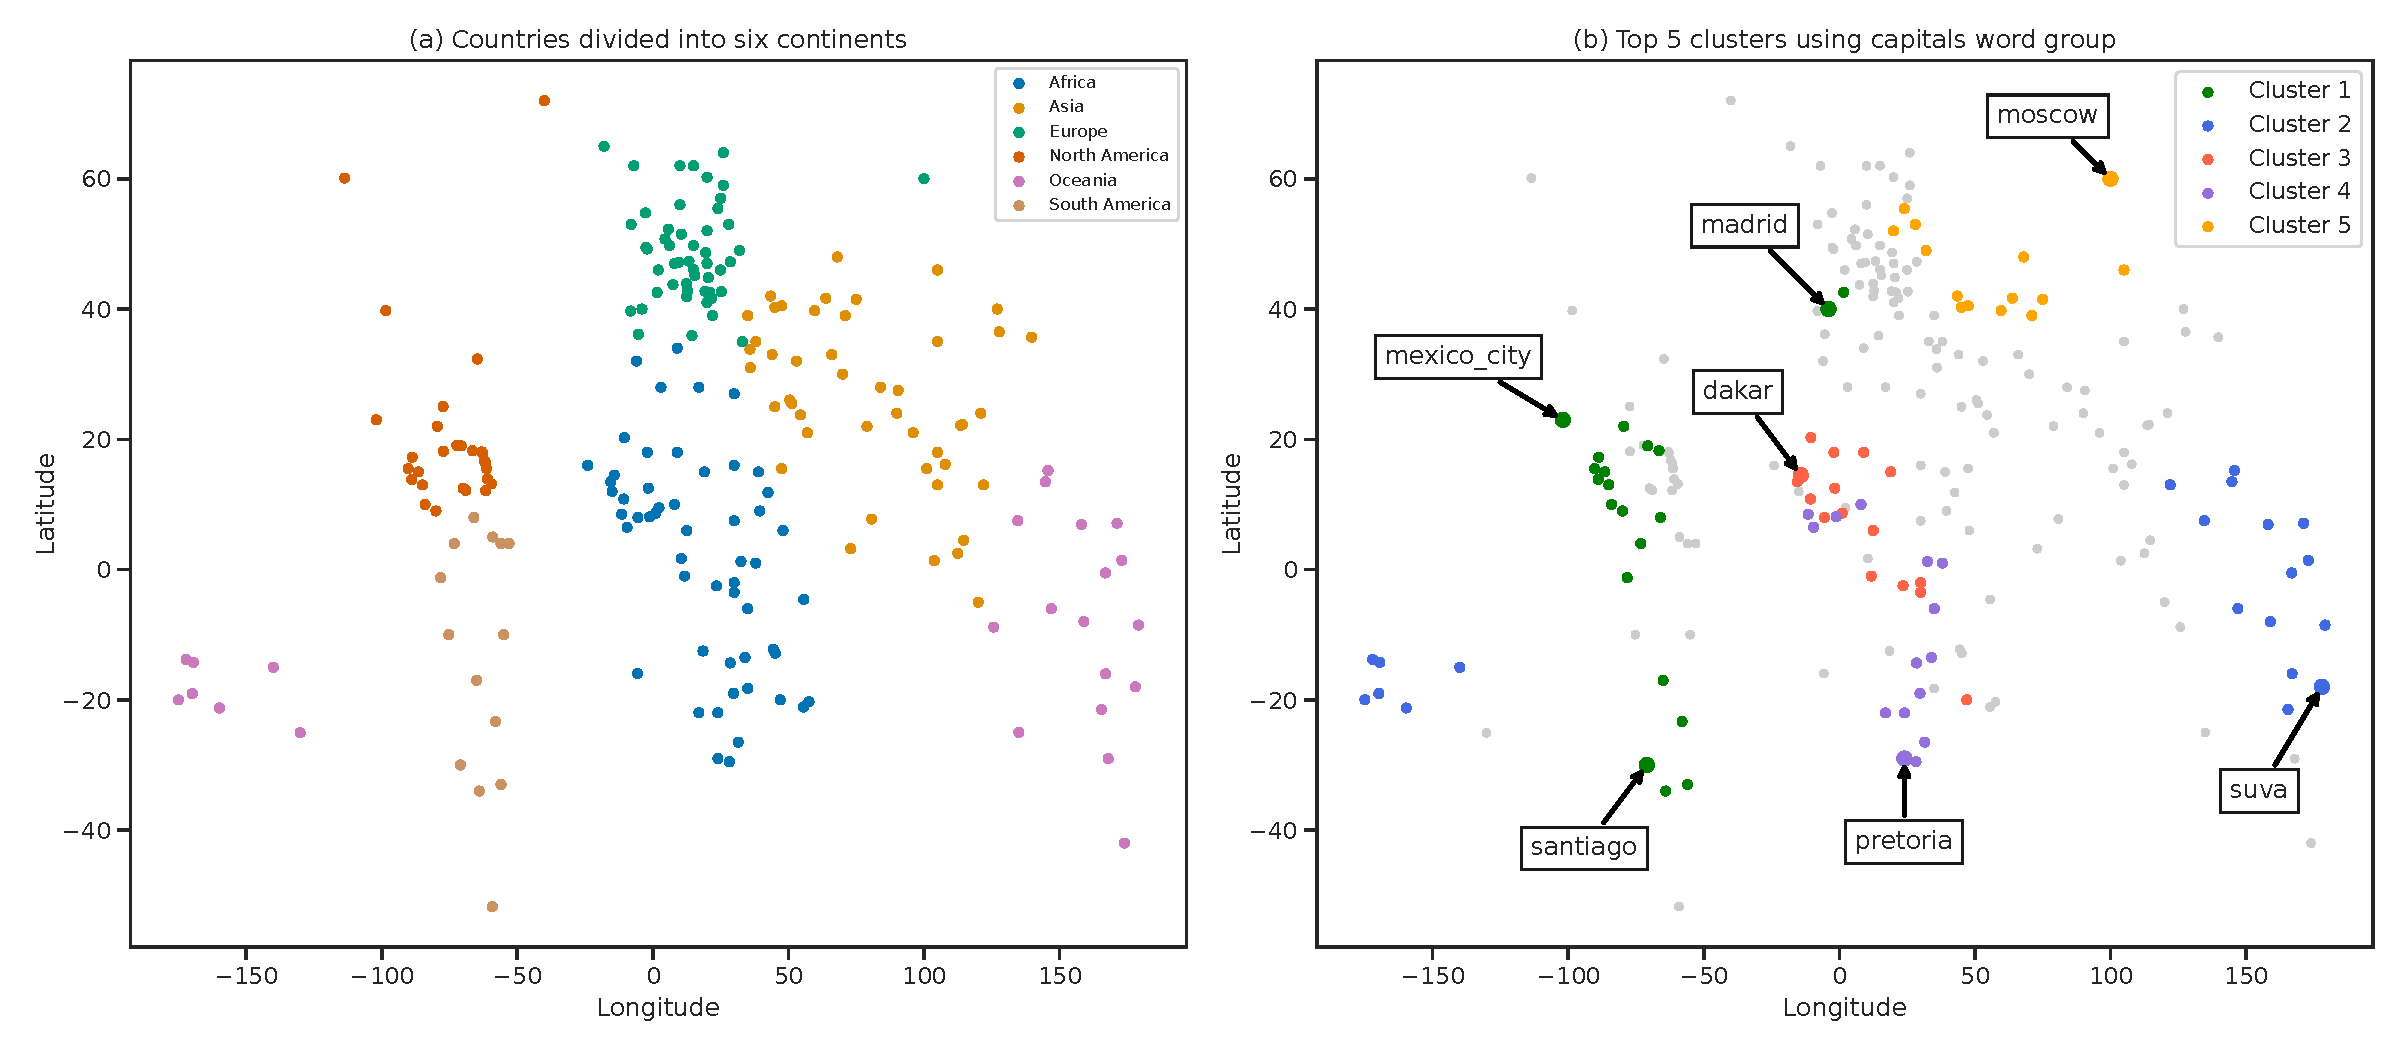
\includegraphics[width=\textwidth]{thesis/figures/cluster-analysis-agglomerative-country-capitals-word-group-top-clusters.pdf}
    \caption{Comparison of countries clustered into their respective continents (a) versus top 5 largest clusters from clustering of capital word embeddings from SGNS-enwiki using agglomerative clustering and ward criterion. From plot (b) we can see that Spanish speaking countries are clustered together in the first cluster (green), while the other clusters are well clustered with regards to the continent of its country.}
    \label{fig:cluster-analysis-agglomerative-country-capitals-word-group-top-clusters}
\end{figure}

We perform cluster analysis of number word embeddings in a similar manner to the cluster analysis of country/capital word embeddings. First, we compare clustering algorithms using internal cluster validation methods, as shown in \cref{fig:cluster-analysis-numbers-word-group-internal-cluster-validation}. From \cref{fig:cluster-analysis-numbers-word-group-internal-cluster-validation}, we see that, overall, the agglomerative clustering algorithm is the best clustering algorithm, when evaluated using internal validation methods.
\begin{figure}[H]
    \centering
    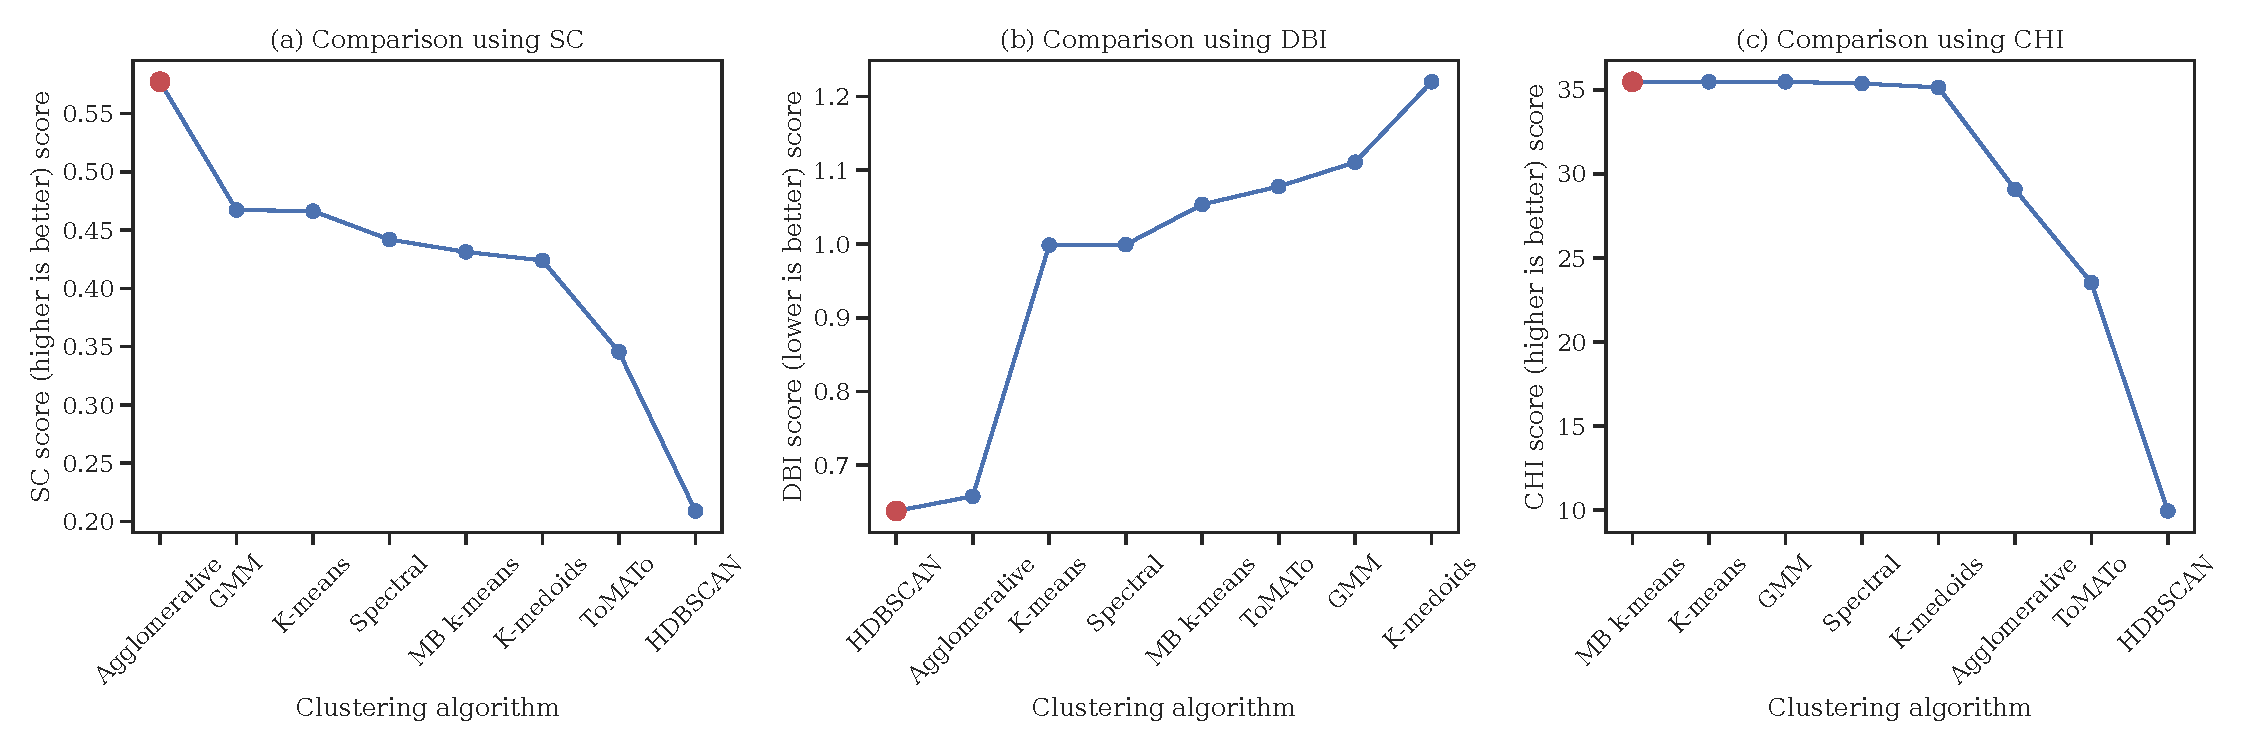
\includegraphics[width=\textwidth]{thesis/figures/cluster-analysis-numbers-word-group-internal-cluster-validation.pdf}
    \caption{Comparison of clustering algorithms trained on number word embeddings from SGNS-enwiki, ranked by internal cluster validation methods. The red dot in each plot denotes the most optimal value.}
    \label{fig:cluster-analysis-numbers-word-group-internal-cluster-validation}
\end{figure}

Furthermore, we use the agglomerative clustering algorithm. To find its best criterion and number of clusters, we first visualize its results in \cref{fig:cluster-analysis-agglomerative-numbers-word-group-internal-cluster-validation}. From \cref{fig:cluster-analysis-agglomerative-numbers-word-group-internal-cluster-validation}, we see that SC (a) prefers complete linkage criterion with 2 clusters, DBI (b) prefers single linkage criterion with 6 clusters and CHI (c) prefers ward linkage criterion with 3 clusters. In other words, we here see a different behaviour of the internal cluster validation methods than in \cref{sec:comparing-clustering-algorithms} and the country/capital cluster analysis, namely that SC prefers the least amount of clusters, DBI does not prefer the most amount of clusters and CHI does not prefer the least amount of clusters.
\begin{figure}[H]
    \centering
    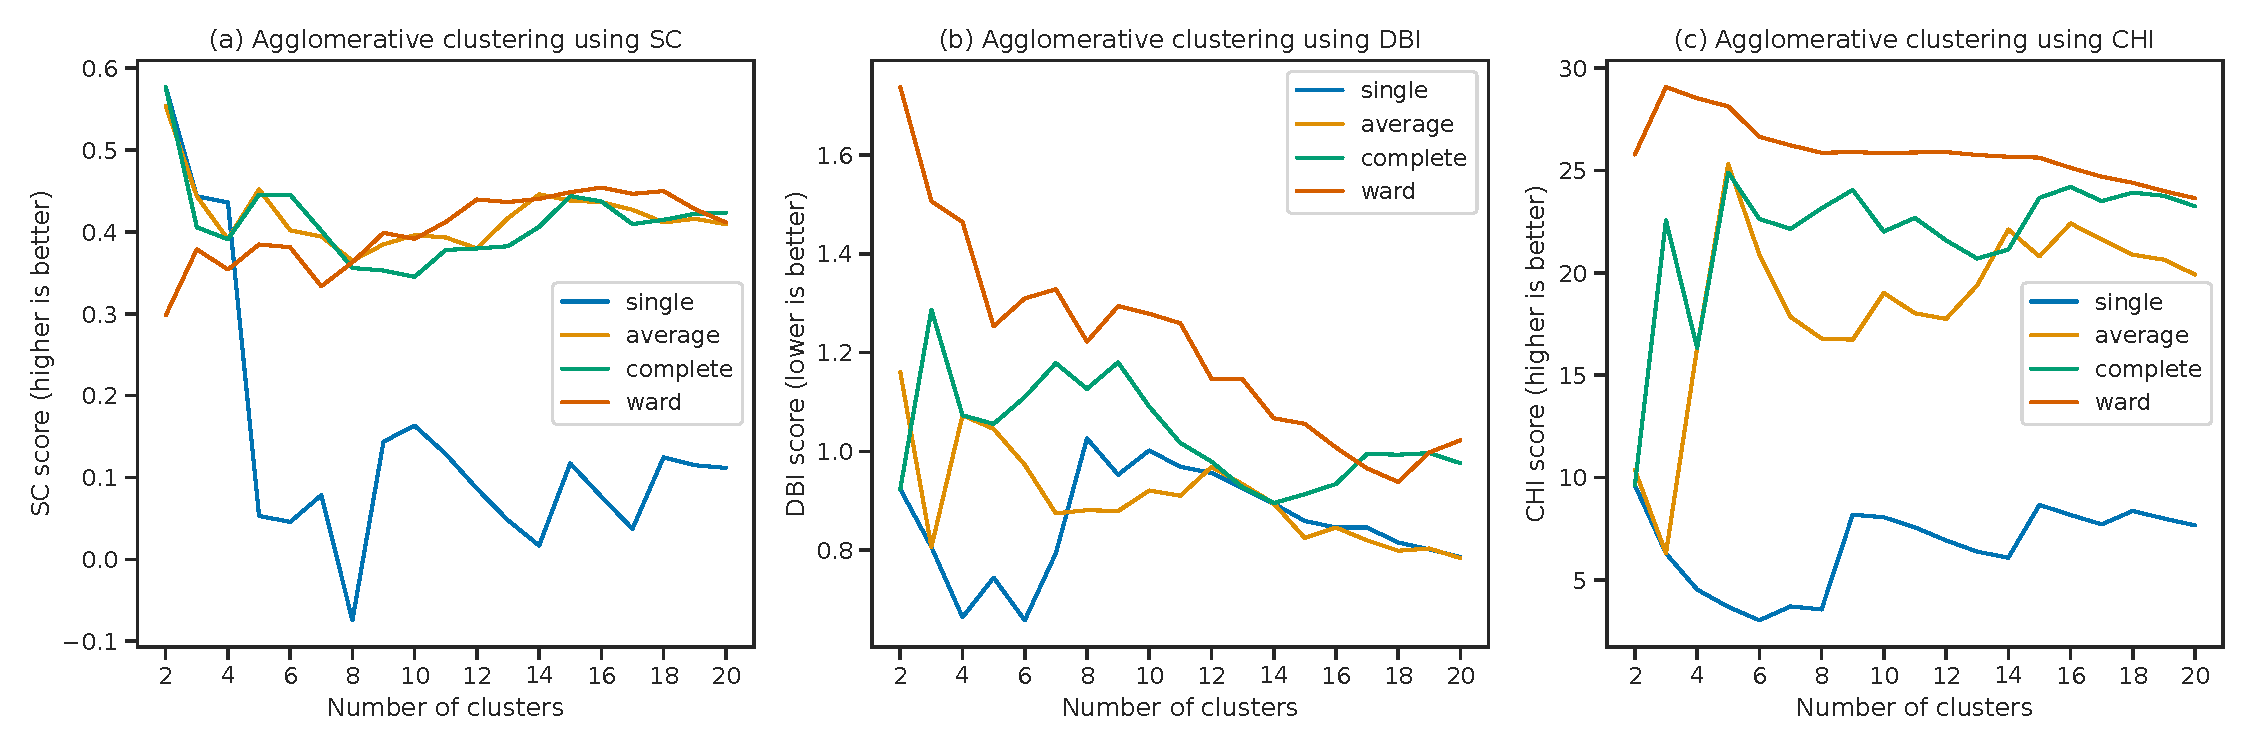
\includegraphics[width=\textwidth]{thesis/figures/cluster-analysis-agglomerative-numbers-word-group-internal-cluster-validation.pdf}
    \caption{Internal cluster validation results using agglomerative clustering on number word embeddings from SGNS-enwiki.}
    \label{fig:cluster-analysis-agglomerative-numbers-word-group-internal-cluster-validation}
\end{figure}

To understand which internal clustering validation method from \cref{fig:cluster-analysis-agglomerative-numbers-word-group-internal-cluster-validation} performs the best, we visualize the result using the best clustering of each of them in three subplots, as show in \cref{fig:cluster-analysis-agglomerative-numbers-word-group-internal-cluster-validation-best-2d-pca}. From \cref{fig:cluster-analysis-agglomerative-numbers-word-group-internal-cluster-validation-best-2d-pca}, we see that it is not entirely clear how to cluster the number word embeddings.
\begin{figure}[H]
    \centering
    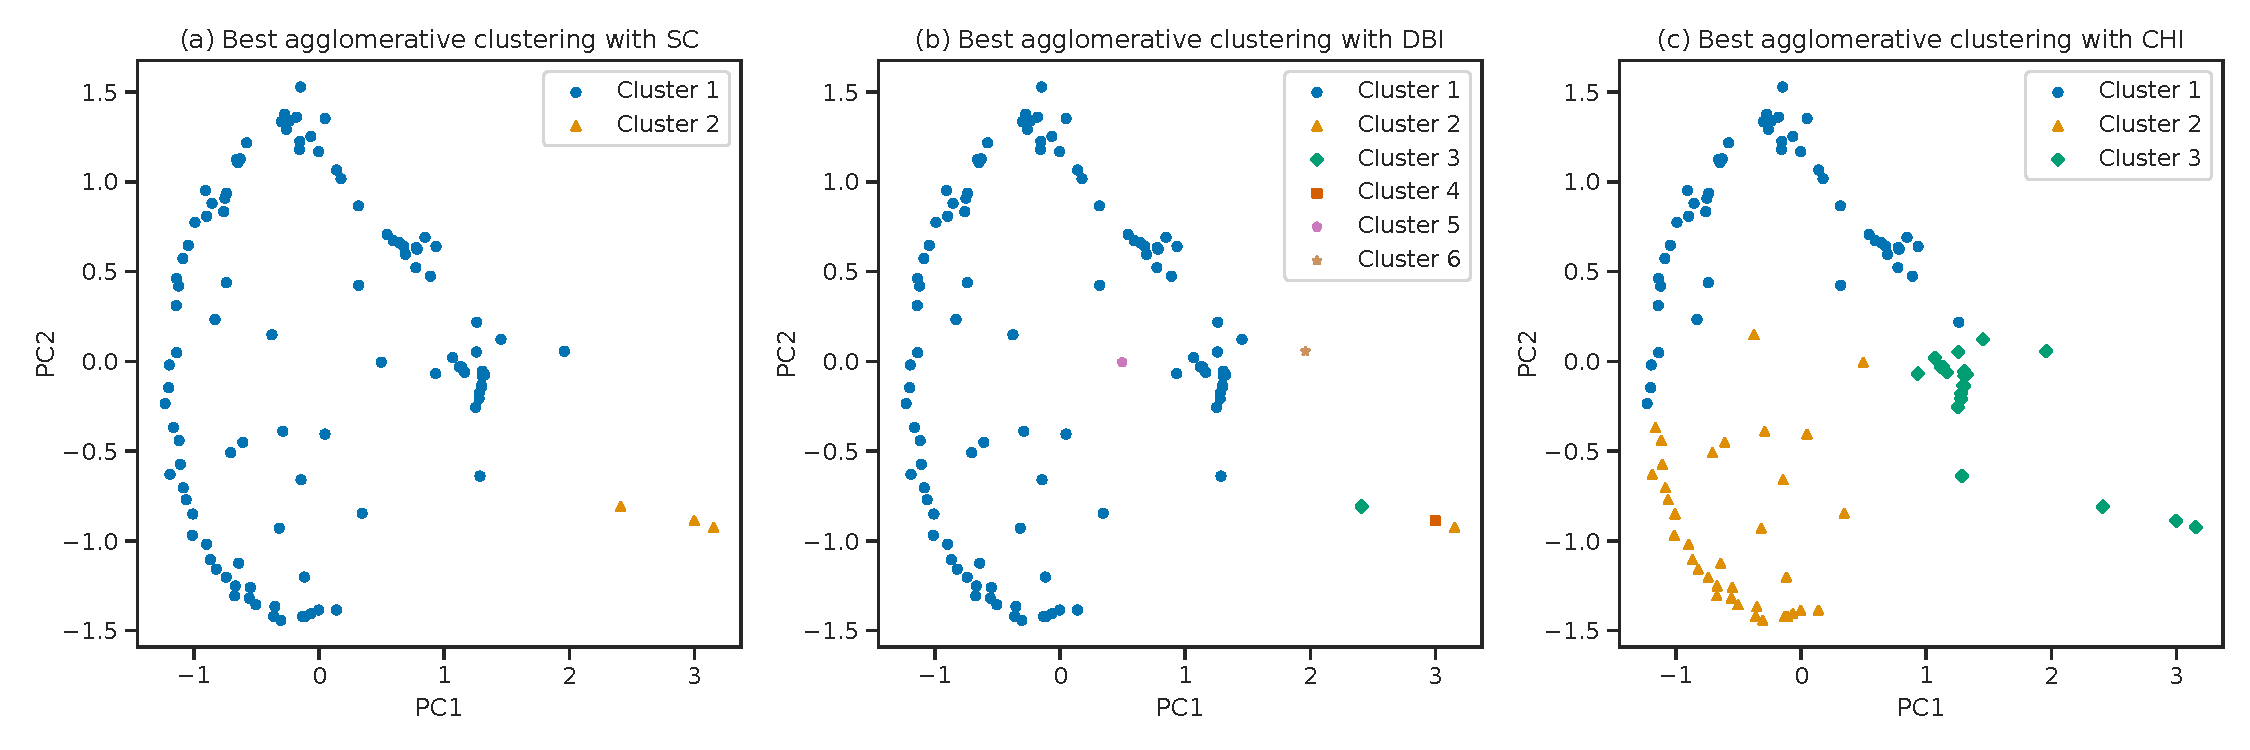
\includegraphics[width=\textwidth]{thesis/figures/cluster-analysis-agglomerative-numbers-word-group-internal-cluster-validation-best-2d-pca.pdf}
    \caption{Comparison of the best result given by internal cluster validation methods using agglomerative clustering on number word embeddings from SGNS-enwiki. Here we see that it is not clear which clustering is the best.}
    \label{fig:cluster-analysis-agglomerative-numbers-word-group-internal-cluster-validation-best-2d-pca}
\end{figure}

We further investigated the structure of the 2-dimensional PCA embedding of the number words, and noticed an interesting relationship. This relationship is illustrated in \cref{fig:ordered-number-word-embeddings-2d-pca} and shows that if we assign an increasing label from the smallest and to the largest number, we see the color of the label gradually increasing from the smallest label color to the largest label color. In other words, there seems to be an underlying sequential relationship to the word embeddings. Furthermore, this suggests that the underlying structure of number word embeddings may contain information which we have not been able to find yet.
\begin{figure}[H]
    \centering
    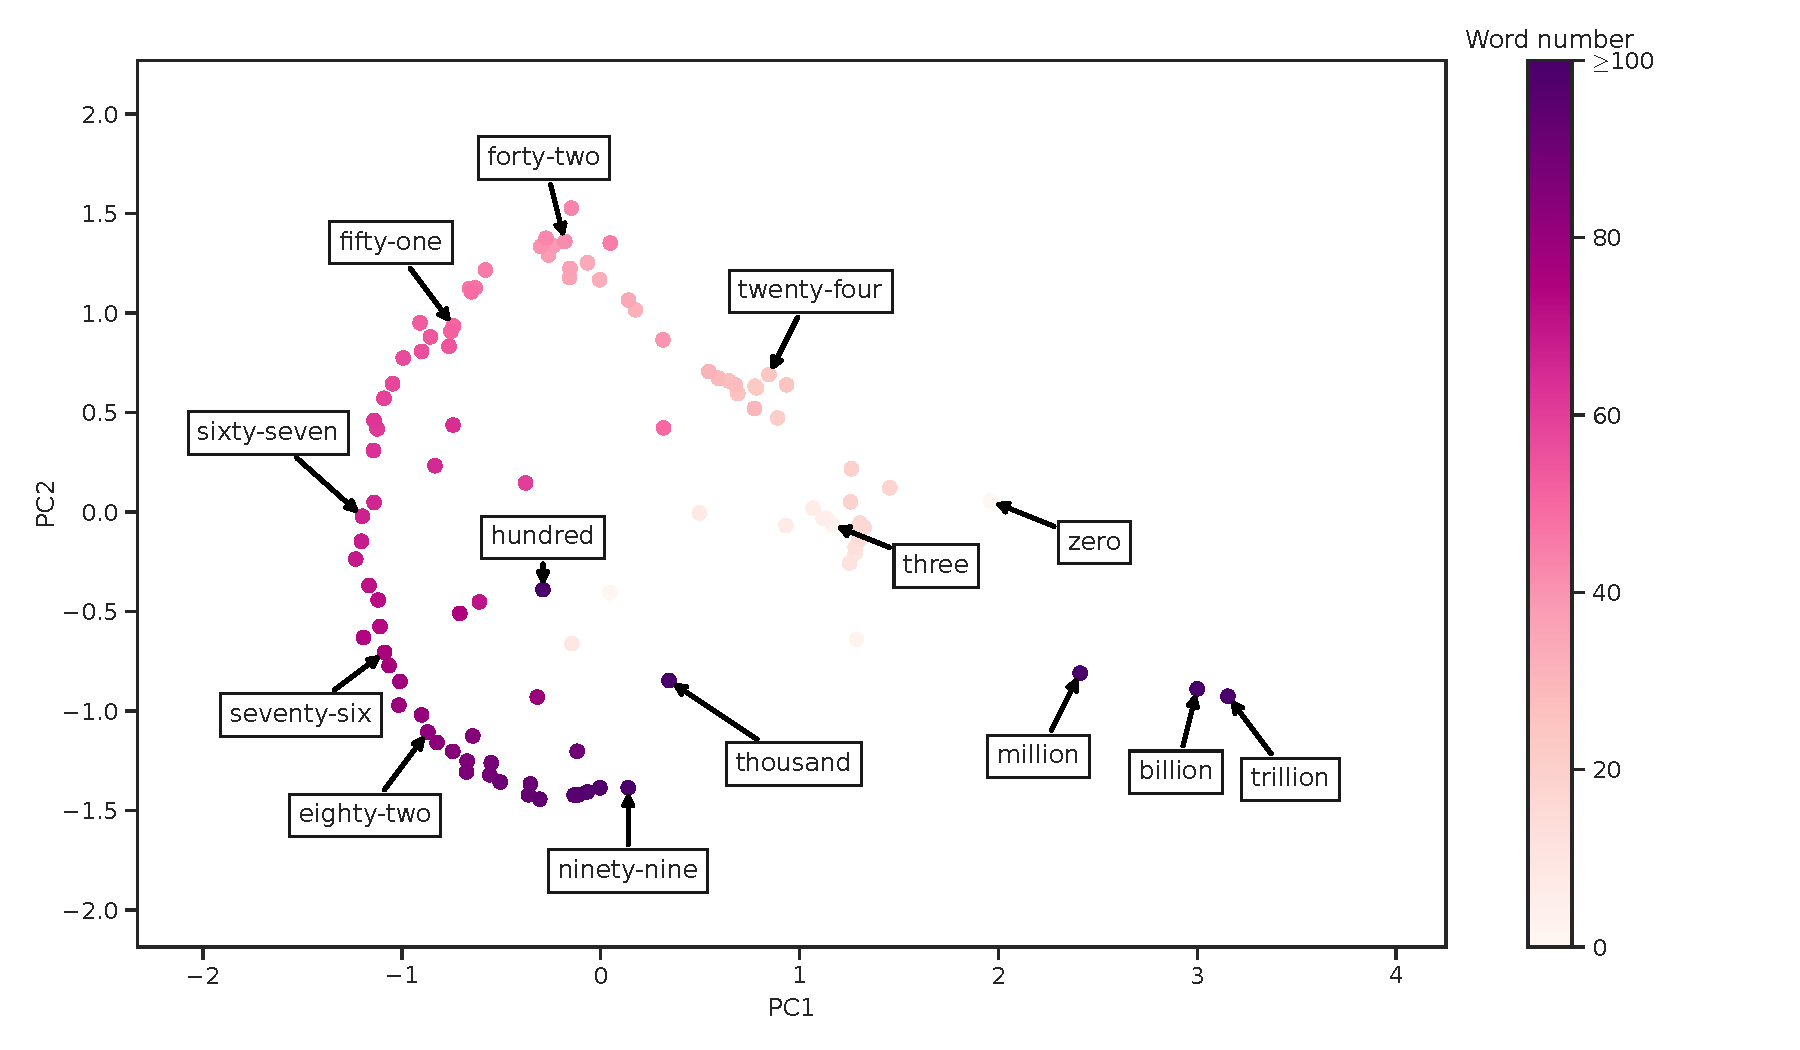
\includegraphics[width=\textwidth]{thesis/figures/ordered-number-word-embeddings-2d-pca.pdf}
    \caption{2-dimensional PCA embedding of the 105 number word embeddings, where each word embedding have an increasing label assigned to it. Here we see that as we increase the number, we see a possible underlying sequential relationship.}
    \label{fig:ordered-number-word-embeddings-2d-pca}
\end{figure}

\section{Polysemous words prediction}
\label{sec:analysis-of-embeddings-tda}
In this section, we try to predict whether or not a word is polysemous, given its word vector. We will, first, apply methods from topological data analysis to word embeddings. In particular, we will investigate the notion of topological polysemy (\cref{sec:topological-polysemy}) and geometric anomaly detection (\cref{sec:geometric-anomaly-detection}). We use topological polysemy to attempt to estimate the number of meanings of a word, given its word vector; we would like to see if the $\text{TPS}_n(w)$ score actually measures polysemy. In addition to this, we would like to see if singular word vectors, as identified by geometric anomaly detection, are polysemous as well. Following, we compute the estimated intrinsic dimension of word embeddings are compare the results with the number of word meanings. Finally, we propose a supervised model to predict the number of word meanings of words.

\subsection{Topological polysemy}
In this subsection, we apply topological polysemy (\cref{sec:topological-polysemy}) to the word embeddings from SGNS-enwiki. We will also train another word2vec model using the same training data used by \cite{jakubowski2020topology} and apply topological polysemy to its word embeddings. We refer to this word2vec model as the \textit{SGNS-semeval} model. Furthermore, we compare the results to topological polysemy applied to word embeddings from pre-trained models, namely the \textit{GoogleNews-vectors-negative300} (shortened to \textit{GoogleNews300}) word embeddings from \cite{GoogleCodeArchiveWord2vec}, the \textit{glove.840B.300d} word embeddings from \cite{GloVeProject2014} and the English (\textit{fastText.en.300d}) word embeddings from \cite{grave2018learning}.

The authors of topological polysemy, \cite{jakubowski2020topology}, trained a fastText model on training data from the \textit{SemEval-2010 Task 14: Evaluation Setting for Word Sense Induction \& Disambiguation Systems} \cite{manandhar-klapaftis-2009-semeval}. The training data from the SemEval task consists of several sentences related to 100 polysemous words (50 nouns and 50 verbs). The SemEval data set also includes the number of true meanings (also called \textit{gold standard} or \textit{GS}) for each of the 100 polysemous words, as perceived by humans. To compare with the $\text{TPS}_n(w)$, the authors use the 100 polysemous words, words from the SemEval training data which has a \textit{WordNet} \cite{fellbaum1998} entry and all words in SemEval training data. WordNet is a lexical database of the English language. In particular, it allows for querying nearly any word from the English language and and returns the \textit{synsets} of the word. Synsets of a query word $w$ is a collection of words which have similar meaning as the word $w$. In other words, by querying a word in WordNet, we can get the number of meanings of a word, as perceived by WordNet. Furthermore, the Pearson correlation coefficient \cite{James2013} is computed between $\text{TPS}_n(w)$ and GS, the number of synsets for WordNet words and the word frequency as they appear in the SemEval training data, respectively. The authors show that there is a moderate (positive) correlation between $\text{TPS}_n(w)$ and GS at $n \in \enclc{40, 50, 60}$, a decreasing correlation between $\text{TPS}_n(w)$ and the number of synsets for WordNet words and no correlation between $\text{TPS}_n(w)$ and word frequencies. In our implementation of topological polysemy, we utilized multiprocessing and the ScaNN \cite{scann2020} approximate nearest neighbour algorithm to speed up the computation. We used the \path{ripser} \cite{ctralie2018ripser} pip-package to compute Vietoris–Rips complexes. \textbf{TODO}: Ripser or Gudhi?

We trained the SGNS-semeval model using the training data from the SemEval task and the hyperparameters used to train the SGNS-enwiki model from \cref{sec:word2vec-hyperparameter-choices}. This resulted in a vocabulary size of $\sim$122K words and corpus size of $\sim$67 million for the SGNS-enwiki model. Following, we will compare the results from the experiments of \cite{jakubowski2020topology} by computing topological polysemy at varying levels of $n$ using the word embeddings of SGNS-enwiki and SGNS-semeval. Finally, we compare the results using the SGNS-enwiki and SGNS-semeval word embeddings to the word embeddings of the GoogleNews300, glove.840B.300d and fastText.en.300d models.

The results of computing topological polysemy at varying levels of $n$ using the word embeddings of SGNS-enwiki and SGNS-semeval are shown in \cref{table:tps-n-correlation-sgns-enwiki,table:tps-n-correlation-sgns-semeval}. From \cref{table:tps-n-correlation-sgns-enwiki}, we see that the correlation between $\text{TPS}_n$ and GS is rather stable with respect to $n$. In particular, we notice that the correlation between $\text{TPS}_n$ and GS is negative, suggesting a relationship in the opposite direction of the results from \cite[Table 1]{jakubowski2020topology}. Nonetheless, we see a decreasing correlation when comparing $\text{TPS}_n$ versus the number of WordNet synsets for each word, and a negligible correlation between $\text{TPS}_n$ and word frequencies of the top 10000 most common words. Furthermore, from \cref{table:tps-n-correlation-sgns-semeval}, we observe a decreasing negative correlation (towards zero) between $\text{TPS}_n$ and GS, meaning that the SGNS-semeval model performs worse than the SGNS-enwiki model on this particular task. This may indicate that by training SGNS-semeval on a smaller vocabulary than the vocabulary of SGNS-enwiki we get worse results. Furthermore, we see a a decreasing correlation between $\text{TPS}_n$ and the number of WordNet synsets and a negligible correlation between $\text{TPS}_n$ and word frequencies of the top 10000 most common words. Although the negative correlation between $\text{TPS}_n$ and the number of WordNet synsets is larger for the SGNS-semeval model than the SGNS-enwiki model, it is still not particularly large. In addition to this, we are considering a lot fewer words when computing the correlation in the SGNS-semeval model than the SGNS-enwiki model (see sample size).
\begin{table}[H]
    \centering
    \begin{tabular}{@{}rrrr@{}}
    \toprule
    $n$ & $\text{TPS}_n$ vs. GS & $\text{TPS}_n$ vs. synsets & $\text{TPS}_n$ vs. frequency \\
    \midrule
    \trcolor 10  & -0.353        & -0.077             & \textbf{-0.043}               \\
    40  & \textbf{-0.383}        & -0.181             & -0.041               \\
    \trcolor 50  & -0.380        & -0.190             & -0.041               \\
    60  & -0.381        & -0.196             & -0.040               \\
    \trcolor 100 & -0.380        & \textbf{-0.205}             & -0.033               \\
    \midrule
    \textit{sample size} & 98 & 144 412 & 10 000 \\
    \bottomrule
    \end{tabular}
    \caption{Correlations between $\text{TPS}_n$ and the number of word meanings as perceived by humans (GS), the number of WordNet synsets and the word frequencies of the top 10000 most common words from the SGNS-enwiki model. \textbf{Bold} values indicate the largest (absolute) correlation.}
    \label{table:tps-n-correlation-sgns-enwiki}
\end{table}
\begin{table}[H]
    \centering
    \begin{tabular}{@{}rrrr@{}}
    \toprule
    $n$ & $\text{TPS}_n$ vs. GS & $\text{TPS}_n$ vs. synsets & $\text{TPS}_n$ vs. frequency \\
    \midrule
    \trcolor 10  & \textbf{-0.300}        & -0.248             & 0.102                \\
    40  & -0.201        & -0.300             & \textbf{0.120}                \\
    \trcolor 50  & -0.194        & -0.304             & 0.116                \\
    60  & -0.169        & -0.306             & 0.110                \\
    \trcolor 100 & -0.130        & \textbf{-0.310}             & 0.098                \\
    \midrule
    \textit{sample size} & 100 & 62 111 & 10 000 \\
    \bottomrule
    \end{tabular}
    \caption{Correlations between $\text{TPS}_n$ and the number of word meanings as perceived by humans (GS), the number of WordNet synsets and the word frequencies of the top 10000 most common words from the SGNS-semeval model. \textbf{Bold} values indicate the largest (absolute) correlation.}
    \label{table:tps-n-correlation-sgns-semeval}
\end{table}

To further broaden our understanding of the results from computing topological polysemy of the word embeddings of the SGNS-enwiki and the SGNS-semeval model, we plot $\text{TPS}_n(w)$ against the GS, the number of WordNet synsets and word frequencies, as shown in \cref{fig:tps-n-correlation-sgns-enwiki,fig:tps-n-correlation-sgns-semeval}. For each plot, we let $n$ be equal to the most optimal value for each column in \cref{table:tps-n-correlation-sgns-enwiki,table:tps-n-correlation-sgns-semeval}. From \cref{table:tps-n-correlation-sgns-enwiki}, we see a similar situation to the results from \cite[Figures 8 and 9]{jakubowski2020topology}, namely that in plot (a) we see an indication of a linear relationship between $\text{TPS}_n(w)$ and the SemEval gold standard and in plot (b) we see a clear trend between $\text{TPS}_n(w)$ and the number of synsets in WordNet. In plot (c) it is clear that there is no apparent relationship between $\text{TPS}_n(w)$ and the word frequencies. Following, we see a similar situation appearing in \cref{table:tps-n-correlation-sgns-enwiki}. These results suggest that, even by computing $\text{TPS}_n(w)$ of the SGNS-enwiki word embeddings, which has a vocabulary much larger than in the experiments of \cite{jakubowski2020topology}, we are unable to use $\text{TPS}_n(w)$ alone for predicting the number of word meanings, as given by the number of WordNet synsets.
\begin{figure}[H]
    \centering
    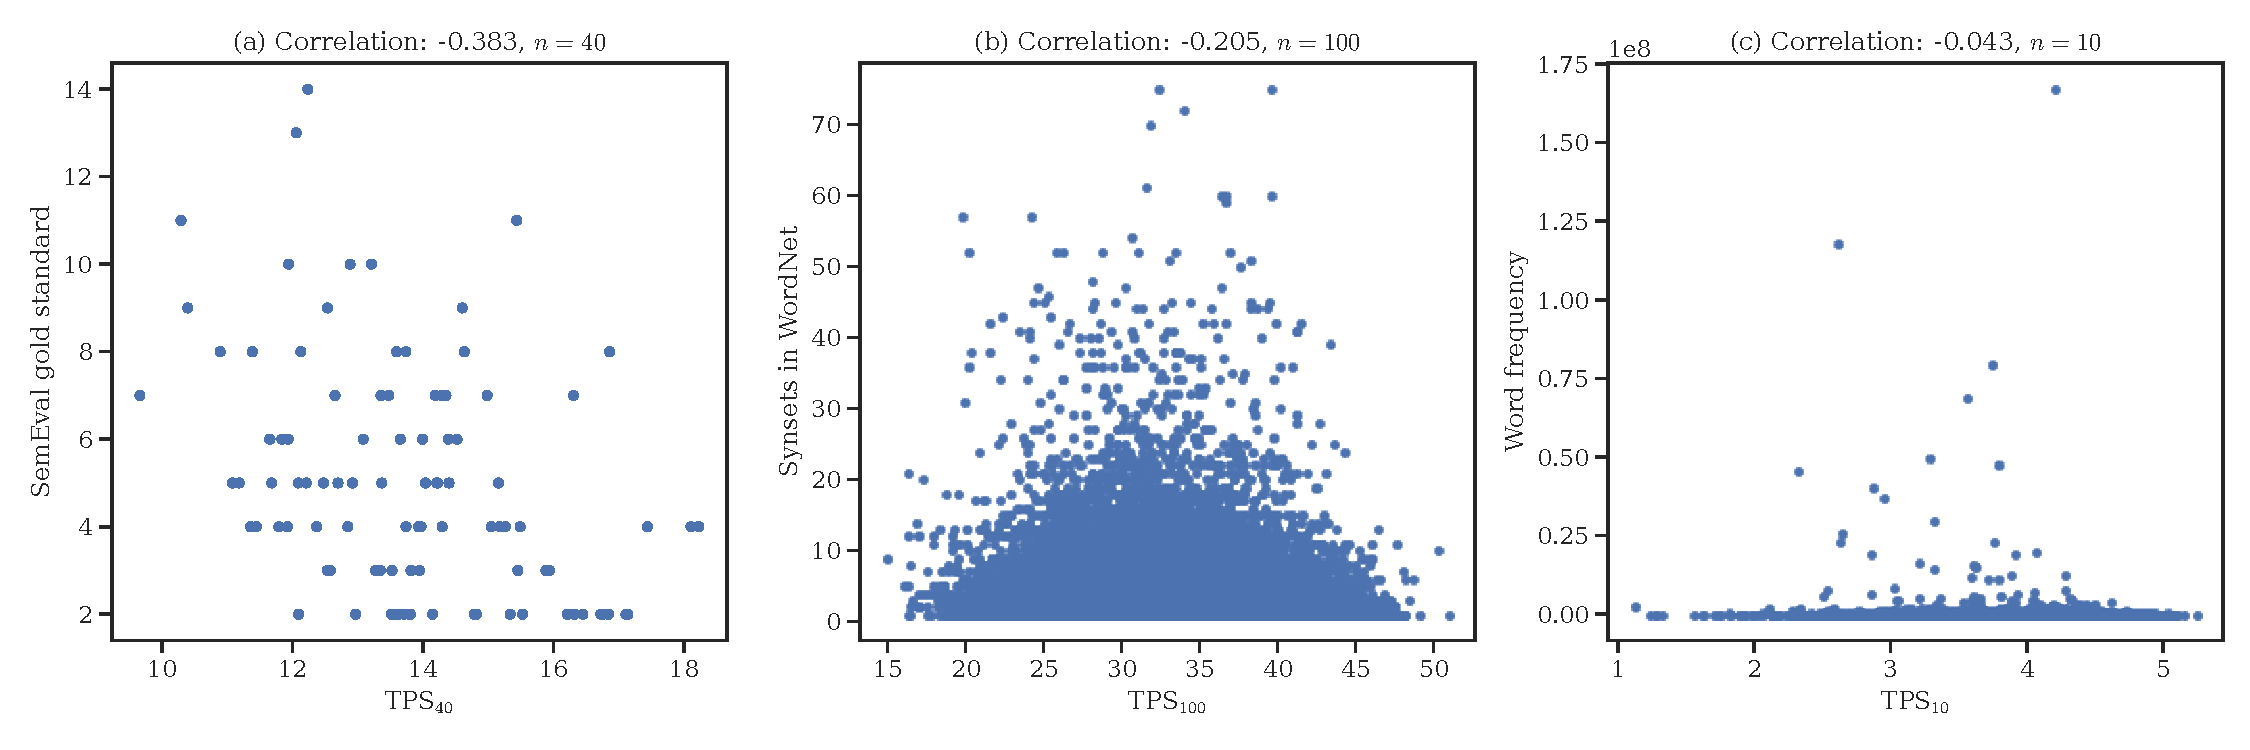
\includegraphics[width=\textwidth]{thesis/figures/tps-n-correlation-sgns-enwiki.pdf}
    \caption{Topological polysemy $\text{TPS}_n(w)$ of the word embeddings of SGNS-enwiki plotted against the GS (a), the number of WordNet synsets (b) and word frequencies (c). Plots are inspired by \cite[Figures 8 and 9]{jakubowski2020topology}.}
    \label{fig:tps-n-correlation-sgns-enwiki}
\end{figure}
\begin{figure}[H]
    \centering
    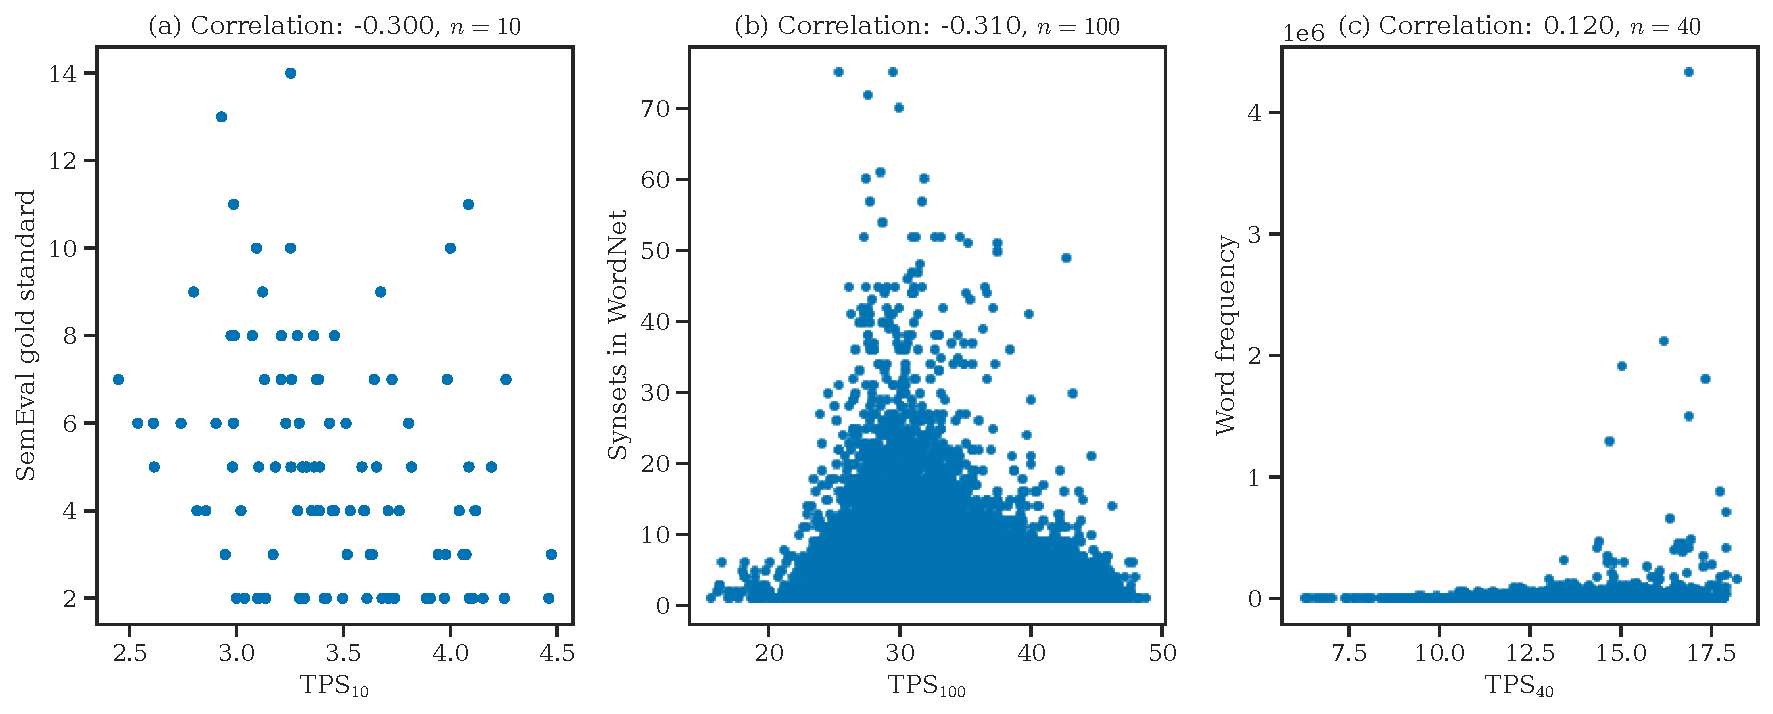
\includegraphics[width=\textwidth]{thesis/figures/tps-n-correlation-sgns-semeval_2010_task_14.pdf}
    \caption{Topological polysemy $\text{TPS}_n(w)$ of the word embeddings of SGNS-semeval plotted against the GS (a), the number of WordNet synsets (b) and word frequencies (c). Plots are inspired by \cite[Figures 8 and 9]{jakubowski2020topology}.}
    \label{fig:tps-n-correlation-sgns-semeval}
\end{figure}

Following, we compare the results of computing $\text{TPS}_n(w)$ of the word embeddings of the SGNS-enwiki and SGNS-semeval models to the word embeddings of the GoogleNews300, glove.840B.300d and fastText.en.300d models. The $\text{TPS}_n(w)$ results of using the GoogleNews300, glove.840B.300d and fastText.en.300d models are shown in \cref{table:tps-n-correlation-external-word-embeddings}. We do not compute the correlation between $\text{TPS}_n(w)$ and word frequencies in \cref{table:tps-n-correlation-external-word-embeddings}, since we do not have the data available. In addition to this, it is unlikely that $\text{TPS}_n(w)$ and word frequencies have anything in common, as show in the previous results using the SGNS-enwiki and SGNS-semeval models, as well as by the experiments of \cite{jakubowski2020topology}. Furthermore, from \cref{table:tps-n-correlation-external-word-embeddings} we see that the GoogleNews300 models yields particularly high values when comparing $\text{TPS}_n(w)$ to the SemEval gold standard, while the remaining models are modest at best. We also observe that when comparing $\text{TPS}_n(w)$ to the number of WordNet synsets, we do not get high correlation scores. This further suggests that by only increasing the vocabulary of the word embedding model, we are not able to model the number of WordNet synsets very well, by only using the $\text{TPS}_n(w)$ scores.
\begin{table}[H]
    \centering
    \begin{tabular}{ccccccc}
    \toprule
    \multicolumn{1}{c}{\multirow{2}{*}{$n$}} & \multicolumn{2}{c}{GoogleNews300}                         & \multicolumn{2}{c}{glove.840B.300d}              & \multicolumn{2}{c}{fastText.en.300d}             \\ \cmidrule(l){2-7} 
    \multicolumn{1}{c}{}                   & \makecell[tc]{$\text{TPS}_n$ vs.\\GS} & \makecell[tc]{$\text{TPS}_n$ vs.\\synsets} & \makecell[tc]{$\text{TPS}_n$ vs.\\GS} & \makecell[tc]{$\text{TPS}_n$ vs.\\synsets} & \makecell[tc]{$\text{TPS}_n$ vs.\\GS} & \makecell[tc]{$\text{TPS}_n$ vs.\\synsets} \\ \midrule
    \trcolor 10           & \textbf{-0.446}  & -0.095       & -0.103  & 0.008        & -0.240  & \textbf{0.114}        \\
    40           & \textbf{-0.446}  & -0.166       & \textbf{-0.125}  & -0.039       & \textbf{-0.289}  & 0.110        \\
    \trcolor 50           & -0.436  & -0.174       & -0.053  & -0.044       & -0.199  & 0.108        \\
    60           & -0.428  & -0.180       & -0.023  & -0.048       & -0.150  & 0.105        \\
    \trcolor 100          & -0.417  & \textbf{-0.193}       & -0.053  & \textbf{-0.058}       & -0.105  & 0.099        \\
    \midrule
    \makecell[tc]{\textit{sample}\\\textit{size}} & 100 & 207 119 & 100 & 249 352 & 100 & 230 175 \\
    \bottomrule
    \end{tabular}
    \caption{Correlations between $\text{TPS}_n$ and the number of word meanings as perceived by humans (GS), and the number of WordNet synsets from the GoogleNews300, glove.840B.300d and fastText.en.300d models. \textbf{Bold} values indicate the largest (absolute) correlation.}
    \label{table:tps-n-correlation-external-word-embeddings}
\end{table}

To compare how well the various word embedding models agree on the $\text{TPS}_n(w)$, we will create a correlation matrix by comparing $\text{TPS}_n(w)$ and the SemEval gold standard. Using a correlation matrix, we summarize the results nicely and further deepen our understanding of the results. By majority vote, we will let $n=40$ when comparing $\text{TPS}_n(w)$ and the SemEval gold standard. The correlation matrix is shown in \cref{fig:correlation-matrix-tps-vs-gs}. From \cref{fig:correlation-matrix-tps-vs-gs}, we see that the SGNS-enwiki, SGNS-semeval and GoogleNews300 models yield similar $\text{TPS}_{40}(w)$ results. We visualize the similarity of the SGNS-enwiki, SGNS-semeval and GoogleNews300 models in \cref{fig:tps-vs-gs-top-3-correlation-word-embedding-models}, where we can see linear relationships appearing. These results suggest that the SGNS-enwiki, SGNS-semeval and GoogleNews300 models perform the best when comparing $\text{TPS}_n(w)$ versus the SemEval gold standard.
\begin{figure}[H]
    \centering
    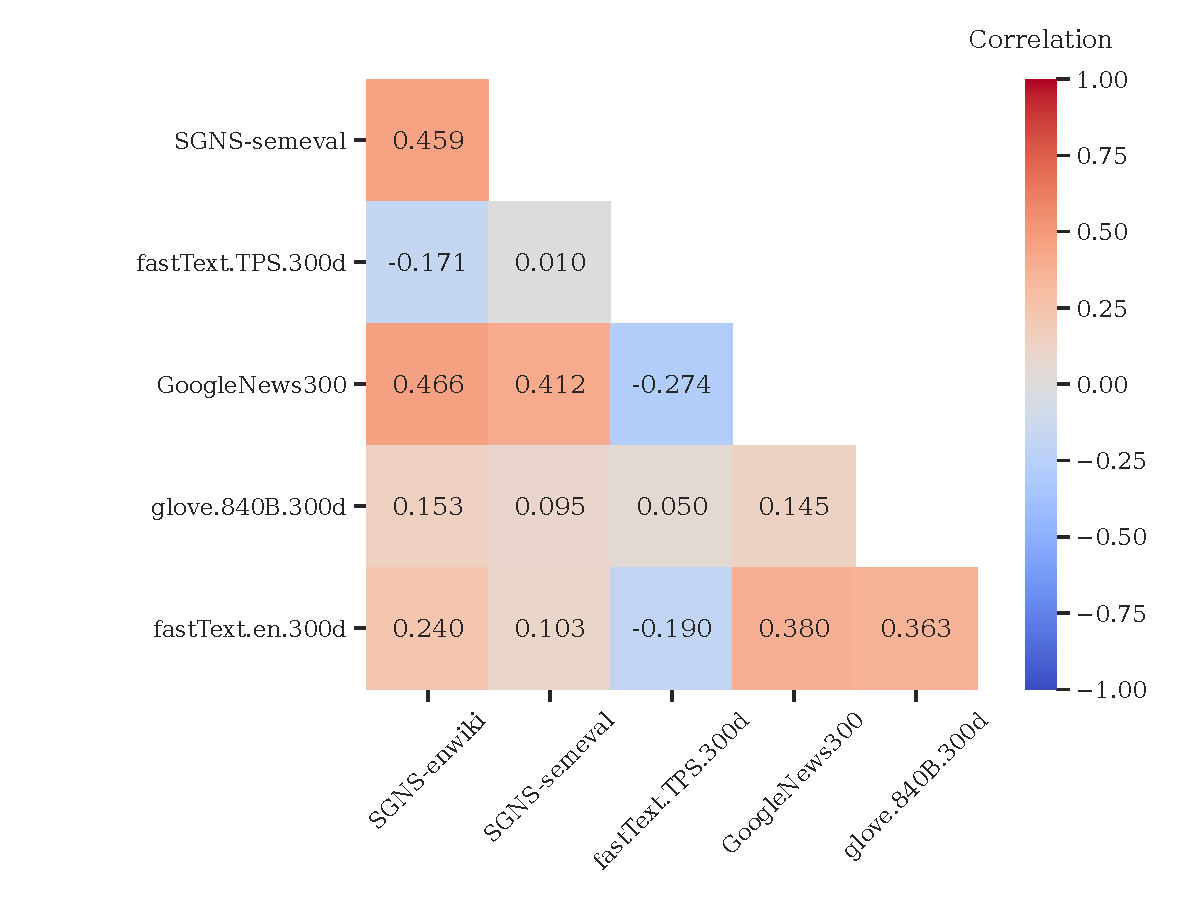
\includegraphics[width=0.8\textwidth]{thesis/figures/correlation-matrix-tps-vs-gs.pdf}
    \caption{Correlation matrix between for comparing word embedding models on correlations between $\text{TPS}_{40}(w)$ and the SemEval gold standard. High (absolute) values indicate that the two models are similar in terms of scoring using $\text{TPS}_{40}(w)$.}
    \label{fig:correlation-matrix-tps-vs-gs}
\end{figure}
\begin{figure}[H]
    \centering
    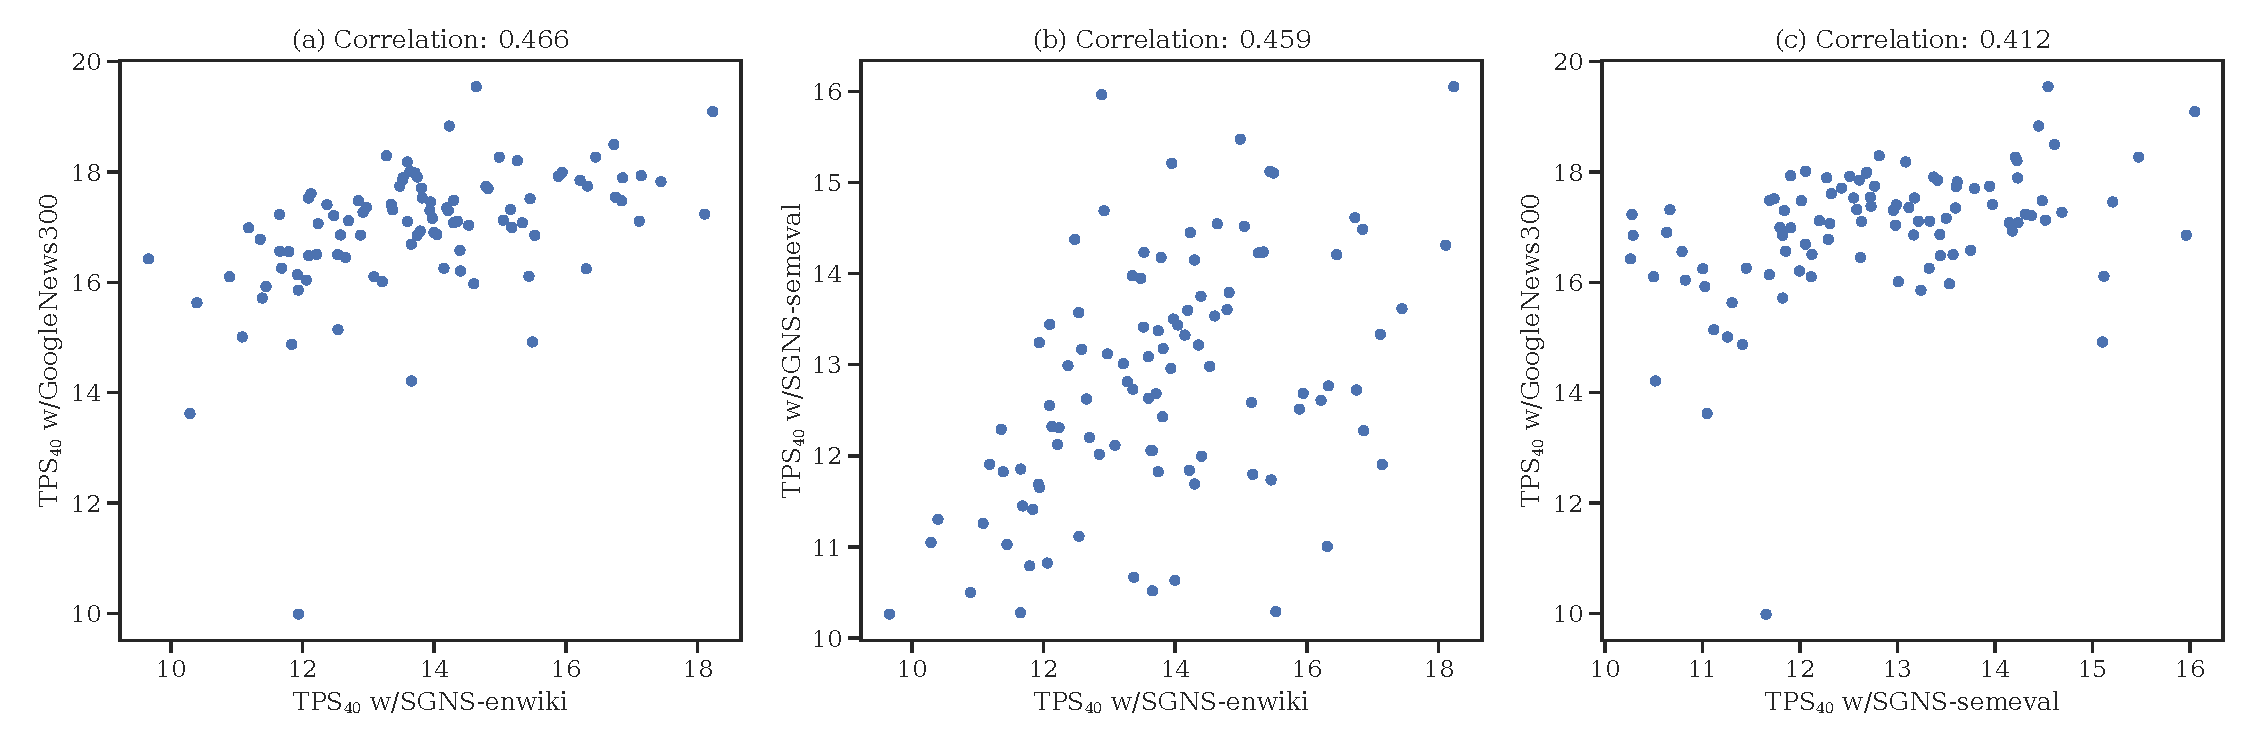
\includegraphics[width=\textwidth]{thesis/figures/tps-vs-gs-top-3-correlation-word-embedding-models.pdf}
    \caption{$\text{TPS}_{40}(w)$ scores plotted against each other using the SGNS-enwiki, SGNS-semeval and GoogleNews300 models.}
    \label{fig:tps-vs-gs-top-3-correlation-word-embedding-models}
\end{figure}

We have now looked at the effect of computing $\text{TPS}_n(w)$ at varying levels of $n$ using various word embeddings. We saw that, even by decreasing/increasing the vocabulary size of the word embedding models, the $\text{TPS}_n(w)$ score did not improve significantly. In all our experiments, the correlation between $\text{TPS}_n(w)$ and the SemEval gold standard were always negative, while in the experiments of \cite{jakubowski2020topology}, they got a moderate, positive correlation. This suggests that the topological polysemy scoring could be affected by choice of word embedding model (i.e. choosing fastText over word2vec) and the fact that the model used in \cite{jakubowski2020topology} was trained on a data set which is strongly related to the 100 polysemous words. In other words, it could seem that the measure of topological polysemy does not work well, for a general word embedding model.

To deepen our understanding of how the $\text{TPS}_n(w)$ is computed, we will perform an experiment by computing $\text{TPS}_n(w)$ of a custom data set. The custom data set consists of sampled data points of two spheres which share one intersection point. We denote this data set as \textit{2Spheres-$d$}, where $d$ represents the dimensionality of the spheres. In particular, we let $d \in \enclc{2, 3, 4, 5, 10, 20, 50, 300}$. To ensure that the dimensionality of the \textit{2Spheres-$d$} data set is similar to the dimensionality of word embeddings, we let the dimensionality of the space be equal to 300, i.e. \textit{2Spheres-$d$} $\in \R^{300}$. In other words, if $d$ was less than 300, we simply add zeros to the remaining dimensions to fill up to 300. For each sphere in \textit{2Spheres-$d$}, we generate 1000000 points on the sphere in $\R^d$. We sort the points by distance to the intersection point and further split the points into 20 intervals, i.e. chunks of 100000 data points for each sphere. Next, we sample 1000 points from each interval, leading to 20000 points for each sphere. The motivation for sampling from distance sorted intervals is to reduce the effect of the curse of dimensionality, namely that it becomes harder to measure the distance between points in high (e.g. 300) dimension. For the sake of simplicity, we let $n=50$ when computing the topological polysemy. We illustrate the result of computing $\text{TPS}_{50}$ of 2Spheres-$2$ and 2Spheres-$3$ in \cref{fig:two-spheres-2d-3d-tps-scores}. From \cref{fig:two-spheres-2d-3d-tps-scores}, we see that for both 2Spheres-$2$ and 2Spheres-$3$, the $\text{TPS}_{50}$ is at its highest (blue color) around the intersection point between the two spheres (see plots (b) and (d)). In addition to this, at the intersection point between the two spheres, the $\text{TPS}_{50}$ score is low. These two observations suggest that, for low values of $d$, $\text{TPS}_{50}$ fails to identify the singular point, but rather manages to identify the area around it. We will now look at how the $\text{TPS}_{50}$ score behaves for $d \in \enclc{4, 5, 10, 20, 50, 300}$.
\begin{figure}[H]
    \centering
    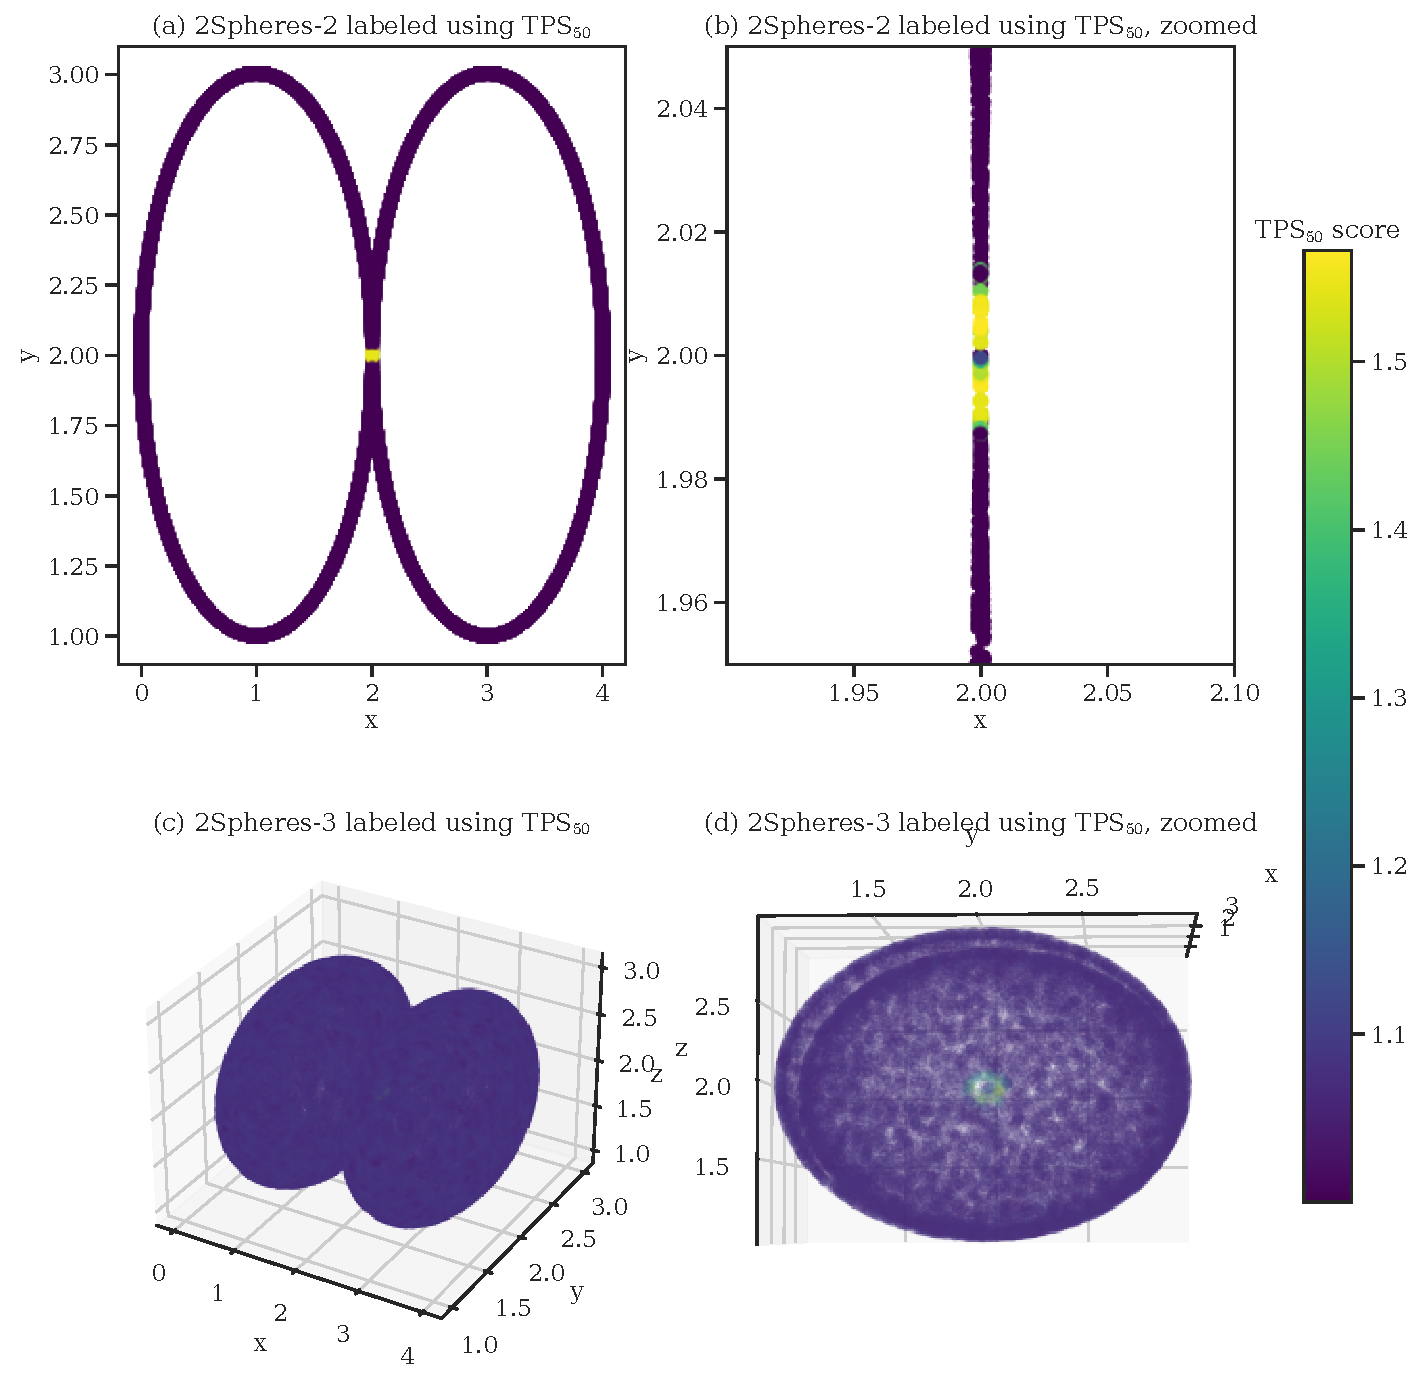
\includegraphics[width=\textwidth]{thesis/figures/two-spheres-2d-3d-tps-scores.pdf}
    \caption{Plots of the 2Spheres-$2$ and 2Spheres-$3$ data sets, with $\text{TPS}_{50}$ as labels.}
    \label{fig:two-spheres-2d-3d-tps-scores}
\end{figure}

We visualize the result of computing $\text{TPS}_{50}$ for 2Spheres-$d$ for $d \in \enclc{4, 5, 10, 20, 50, 300}$ in \cref{fig:two-spheres-distance-to-int-point-vs-tps-scores}, by plotting the distance to intersection point between the spheres against the $\text{TPS}_{50}$ score. From \cref{fig:two-spheres-distance-to-int-point-vs-tps-scores}, we see that as the dimension of the spheres increases, the "peak" of $\text{TPS}_{50}$ shown in plot (a) diminishes. The diminishing effect comes due to the curse of dimensionality (\cref{fig:curse-of-dimensionality}), namely that in high dimensional space, all distances become very similar (as seen in plot (f)). In other words, for high dimensional spheres, it becomes very hard to identify the intersection point using $\text{TPS}_{50}$, as the distances become similar, and $\text{TPS}_{50}$ is unable to identify areas around the intersection point, as we saw happened in lower dimensions (\cref{fig:two-spheres-2d-3d-tps-scores}). It should be noted, however, that for high values of $d$, the intersection point has a $\text{TPS}_{50}$ score which generally is higher than all other values of $\text{TPS}_{50}$. Finally, we conclude that these results shown in \cref{fig:two-spheres-distance-to-int-point-vs-tps-scores} may indicate that the topological measure of polysemy may suffer when applied to high-dimensional (e.g. 300) data.
\begin{figure}[H]
    \centering
    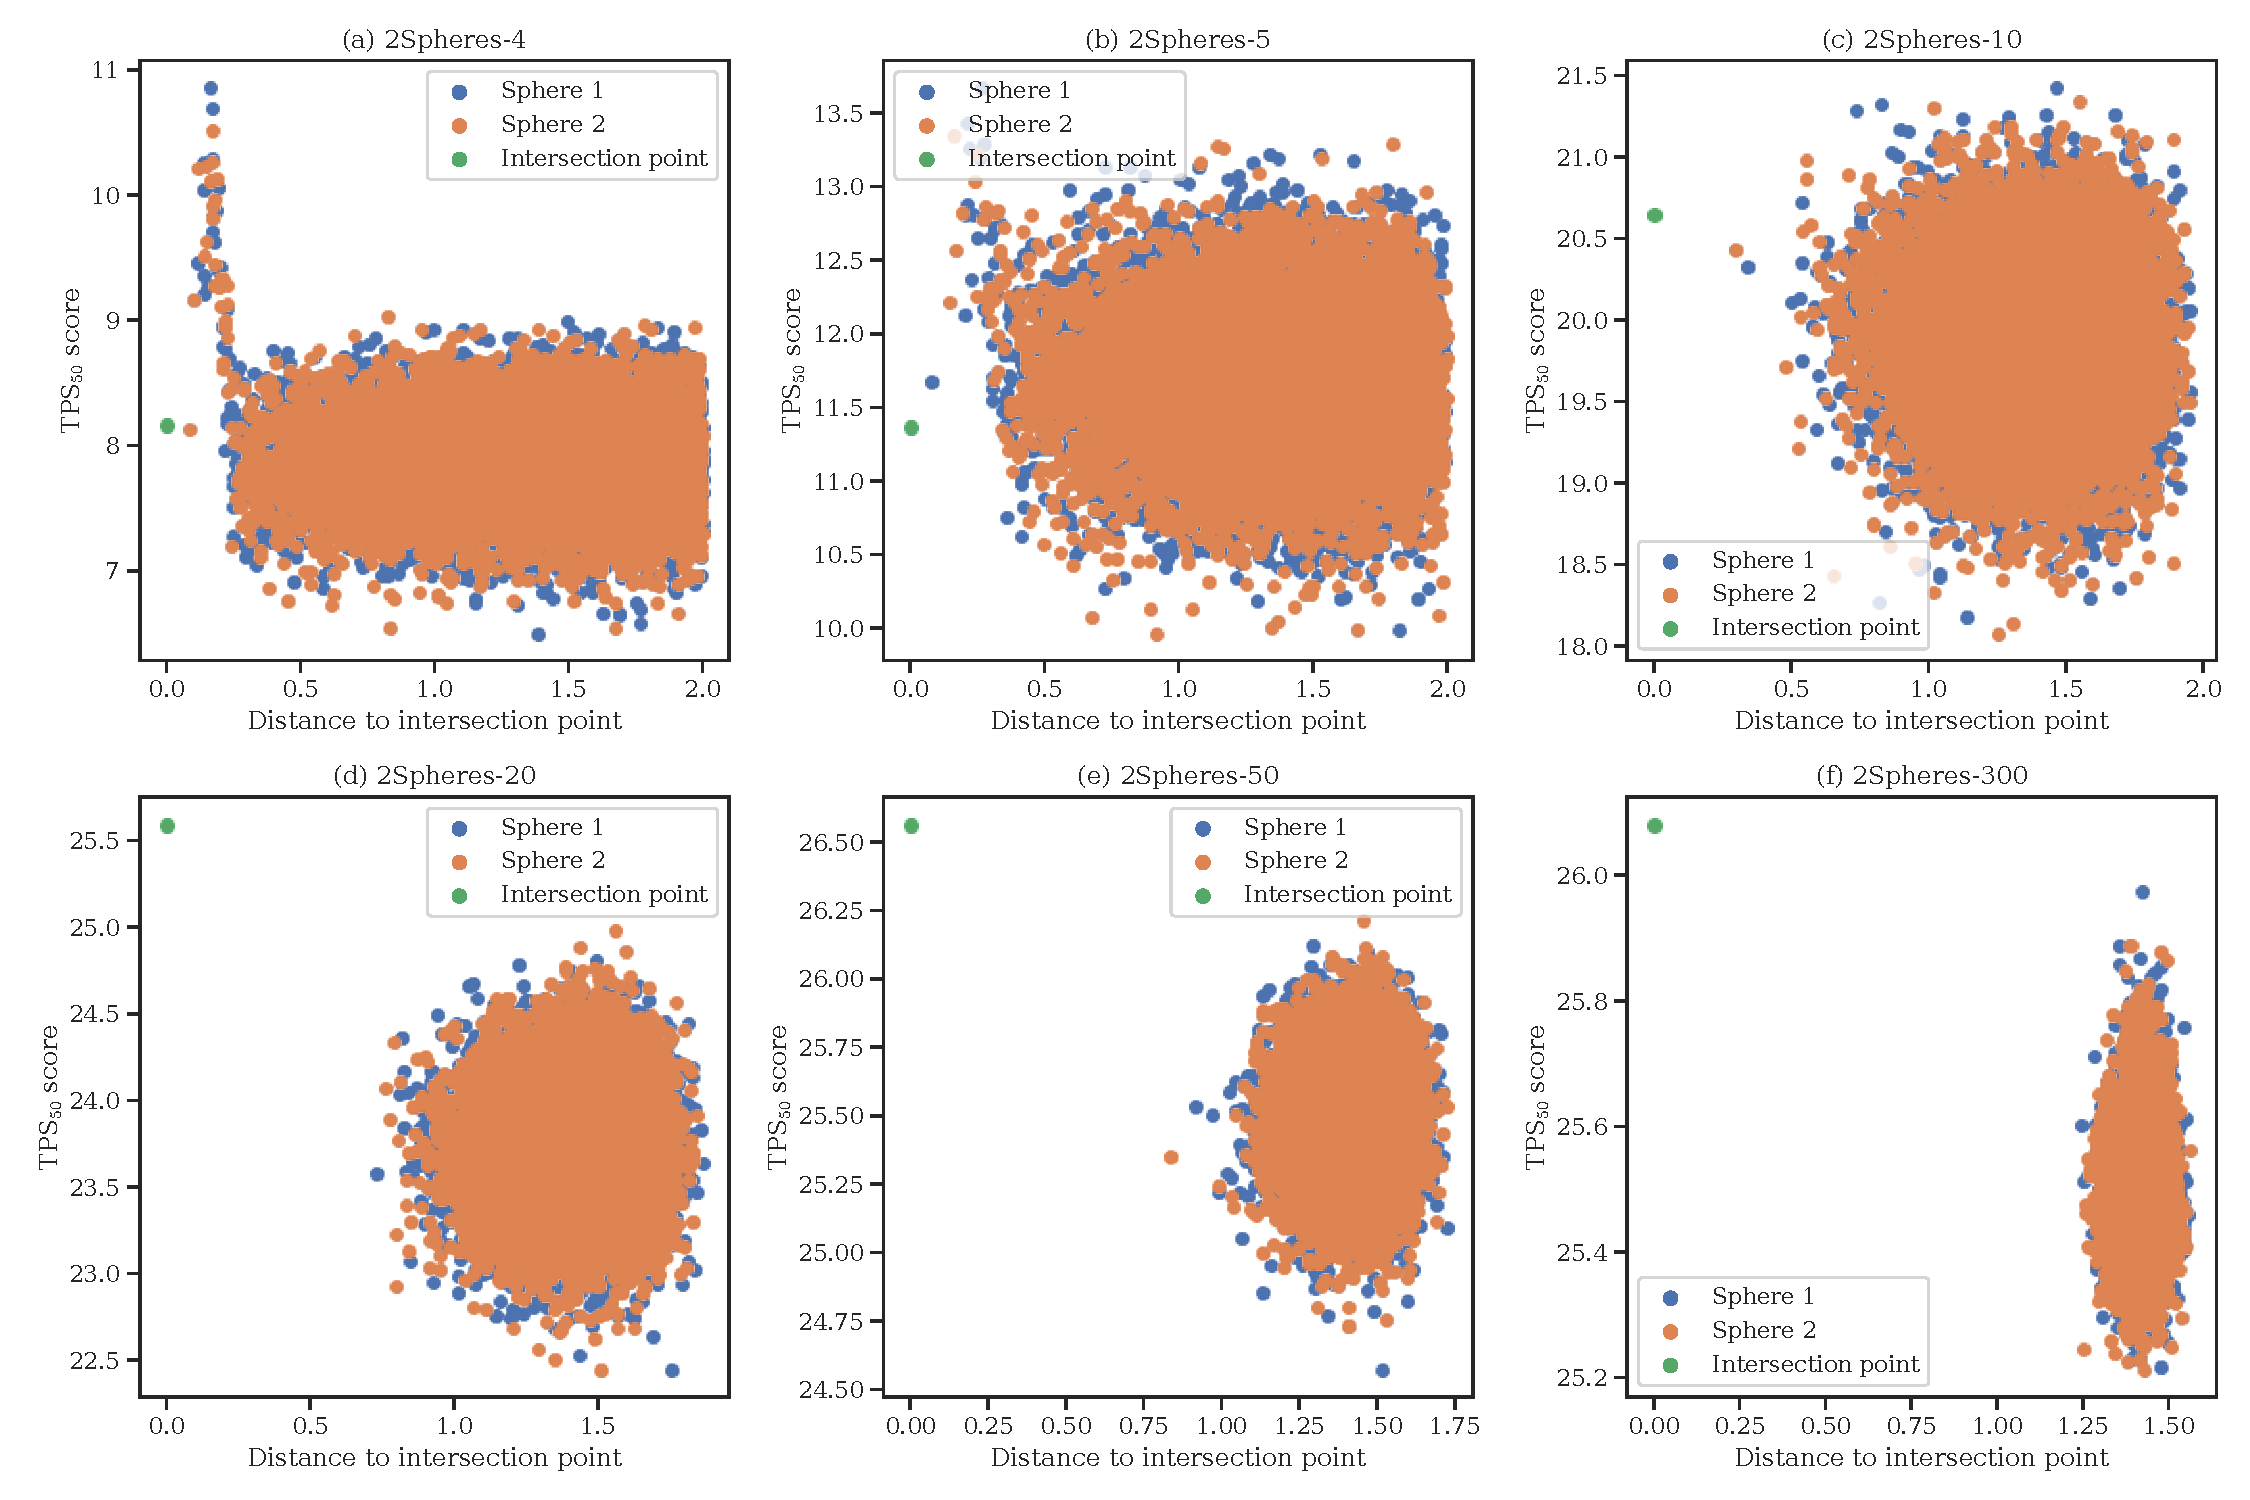
\includegraphics[width=\textwidth]{thesis/figures/two-spheres-distance-to-int-point-vs-tps-scores.pdf}
    \caption{Distance to intersection point between spheres plotted against $\text{TPS}_{50}$ score for 2Spheres-$d$, $d \in \enclc{4, 5, 10, 20, 50, 300}$.}
    \label{fig:two-spheres-distance-to-int-point-vs-tps-scores}
\end{figure}

\textbf{TODO}: Repeat sphere experiment with added noise to spheres.

\subsection{Geometric anomaly detection}
TODO

\subsection{Intrinsic dimension estimation}
TODO: Add correlation figure, etc.

\subsection{Supervised polysemy prediction}
TODO